%\documentclass{article}
%\usepackage[utf8]{inputenc}
%\title{test}
%\author{paolo.dini }
%\date{June 2017}
%\begin{document}
%\maketitle
%\section{Introduction}
%\end{document}

%===================================================
%================== DOCUMENT CLASS
%===================================================
\documentclass[runningheads,11pt,a4paper,english,llncs]{Misc/llncs}

%===================================================
%================== PACKAGES
%===================================================
%------------------------------------------------------------------------
% TeX and LaTeX macros
%------------------------------------------------------------------------
%
% In math formulas we use italic instead of mathitalic
%
\makeatletter
% ~ gives a \; space in math mode
\def~{\ifmmode\;\else\penalty\@M\ \fi}
%  Italic in mathematical formulas
\def\@setmcodes#1#2#3{{\count0=#1 \count1=#3
  \loop \global\mathcode\count0=\count1 \ifnum \count0<#2
  \advance\count0 by1 \advance\count1 by1 \repeat}}
\DeclareSymbolFont{italic}{OT1}{\rmdefault}{m}{it}
\let\mathit\undefined
\DeclareSymbolFontAlphabet{\mathit}{italic}
\edef\@tempa{\hexnumber@\symitalic}
\@setmcodes{`A}{`Z}{"7\@tempa41}
\@setmcodes{`a}{`z}{"7\@tempa61}
\makeatother
%
% \begin{asm} ... \end{asm}
%
\newdimen\asmindent     
\asmindent=\parindent
\newcount\asmi
\def\inc{\global\advance\asmi by 1}
\def\dec{\global\advance\asmi by-1}
\def\nl{{}$\par\hangindent\asmi em
  \noindent\kern\asmi em\ignorespaces$} 
\def\asmskip{{}$\par\smallskip\hangindent\asmi em
  \noindent\kern\asmi em\ignorespaces$} 
\def\asm{\global\asmi=0 
%%%%%%%%%%%%%% added by Paolo:
\parskip=0pt
%%%%%%%%%%%%%%%%%%%%%%%
 \def\+{\inc\nl}
 \def\-{\dec\nl}
 \def\\{\nl}
 \begin{trivlist}\item[]\leftskip=\asmindent\relax$}
\def\endasm{$\end{trivlist}}
%\mathindent=\asmindent
%
% \begin{asmarray}
%    f(s_1) & := t_1 \\
%    f(s_2) & := t_2 
% \end{asmarray}
%
\def\asmarray{\begin{array}[t]{@{}l@{\;}l@{\;}l@{}}}
\def\endasmarray{\end{array}}
%
%
%
\def\asmcomment#1{\quad\hbox{// #1}}
%
%  \begin{subasm} ... \end{subasm}
%
\newcount\asmii
\def\subasm{\vtop\bgroup\asmii=0\normalbaselines
 \def\nl##1{$\egroup\advance\asmii by##1\relax\hbox\bgroup\hskip\asmii em$}
 \def\\{\nl{0}}
 \def\+{\nl{1}}
 \def\-{\nl{-1}}
 \hbox\bgroup\hskip\asmii em$}
\def\endsubasm{$\egroup\egroup}
%
% Keywords in ASM code
%
\def\ASM#1{\hbox{\sc#1}}        % rule names and macros
\def\ASMIND#1{\ASM{#1}\index{#1@{\sc#1}}}
\def\AWAIT   {\mathrel{\mathbf{await}}}
\def\AND     {\mathrel{\mathbf{and}}}
\def\CASE    {\mathrel{\mathbf{case}}}
\def\CHOOSE  {\mathrel{\mathbf{choose}}}
\def\CREATE  {\mathrel{\mathbf{create}}}
\def\NEW  {\mathrel{\mathbf{new}}}
\def\DO      {\mathrel{\mathbf{do}}}
\def\ELSE    {\mathrel{\mathbf{else}}}
\def\ELSEIF  {\mathrel{\mathbf{elseif}}}
\def\FORALL  {\mathrel{\mathbf{forall}}}
\def\FORSOME  {\mathrel{\mathbf{forsome}}}
\def\FOREACH  {\mathrel{\mathbf{foreach}}}
\def\FROM  {\mathrel{\mathbf{from}}}
\def\THEREISNO  {\mathrel{\mathbf{thereisno}}}
\def\IF      {\mathrel{\mathbf{if}}}
\def\IFF      {\mathrel{\mathbf{iff}}}
\def\IMPORT  {\mathrel{\mathbf{import}}}
\def\IN      {\mathrel{\mathbf{in}}}
\def\LET     {\mathrel{\mathbf{let}}}
\def\SELF    {\mathrel{\mathbf{self}}}
\def\MATCH    {\mathrel{\textbf{match}}}
\def\NOT     {\mathrel{\mathbf{not}}}
\def\OF      {\mathrel{\mathbf{of}}}
\def\OR      {\mathrel{\mathbf{or}}}
\def\PAR     {\mathrel{\mathbf{par}}}
\def\SEQ     {\mathrel{\mathbf{seq}}}
\def\SKIP    {\mathrel{\mathbf{skip}}}
\def\THEN    {\mathrel{\mathbf{then}}}
\def\TO  {\mathrel{\mathbf{to}}}
\def\WHERE   {\mathrel{\mathbf{where}}}
\def\WHILE   {\mathrel{\mathbf{while}}}
\def\UNDEF   {\mathrel{\mathbf{undef}}}
\def\UNTIL   {\mathrel{\mathbf{until}}}
\def\WHEN   {\mathrel{\mathbf{when}}}
\def\WITH    {\mathrel{\mathbf{with}}}
\def\STEP    {\mathrel{\mathbf{step}}}
\def\STEPWISE    {\mathrel{\mathbf{stepwise}}}
\def\SEQ    {\mathrel{\mathbf{seq}}}
\def\RESULT  {\mathrel{\mathbf{result}}}
\def\CALL  {\mathrel{\mathbf{Call}}}
\def\LOCAL    {\mathrel{\mathbf{local}}}
\def\ADDGUARD {\mathrel{\mathbf{addGuard}}}
\def\ADDUPD   {\mathrel{\mathbf{addUpd}}}
\def\ADDRULE  {\mathrel{\mathbf{addRule}}}
\def\MINUSRULE  {\mathrel{\mathbf{minusRule}}}
\def\TO      {\mathrel{\mathbf{to}}}
%
% Including figures
%
\def\includefig#1#2{\centering\medskip
  \includegraphics[scale=#1]{fig/#2}
  \medskip}
%
% References to paragraphs in the ECMA standard for C#
%
\def\ecma#1{\cite[\S#1]{ecma334}}
%
%  Environments for definitions and theorems
%
%\theorembodyfont{\rm}
%\newtheorem{definition}[subsection]{Definition}
%\newtheorem{lemma}[subsection]{Lemma}
%\newtheorem{theorem}[subsection]{Theorem}
%\newtheorem{proposition}[subsection]{Proposition}
%\newtheorem{corollary}[subsection]{Corollary}
%\newtheorem{example}[subsection]{Example}
%\newtheorem{remark}[subsection]{Remark}
%\newtheorem{constraint}[subsection]{Constraint}
\def\proof{\trivlist\item[]{\bf Proof.}}
\def\endproof{$\Box$\endtrivlist}
%
% enumerate and itemize (smaller skips) from "latex.ltx"
%
\makeatletter
\def\enumerate{%
  \ifnum \@enumdepth >\thr@@\@toodeep\else
    \advance\@enumdepth\@ne
    \edef\@enumctr{enum\romannumeral\the\@enumdepth}%
      \expandafter
      \list
        \csname label\@enumctr\endcsname
        {\usecounter\@enumctr\def\makelabel##1{\hss\llap{##1}}
         \itemsep 0pt\parskip 0pt\parsep 0pt\topsep\smallskipamount}%
  \fi}
\def\itemize{%
  \ifnum \@itemdepth >\thr@@\@toodeep\else
    \advance\@itemdepth\@ne
    \edef\@itemitem{labelitem\romannumeral\the\@itemdepth}%
    \expandafter
    \list
      \csname\@itemitem\endcsname
      {\def\makelabel##1{\hss\llap{##1}}
       \itemsep 0pt\parskip 0pt\parsep 0pt\topsep\smallskipamount}%
  \fi}
\makeatother
%
% items in itemize
%
\def\bull{\vrule height .9ex width .8ex depth -.1ex}
\def\labelitemi{\bull}
%
%
%
\def\cs#1{C\#$_{\mathcal{#1}}$}
\def\lang#1{L$_{\mathcal{#1}}$}
%
% Positions
%
\def\pos#1{{}^{#1}}
\def\termPos{\blacktriangleright}
\def\cursor{\pos{\termPos}}
%
%
%
\def\sup{\hbox{sup}}
\def\c#1{\texttt{#1}}           % code
\def\N#1{\textit{#1}}           % non terminal symbols
\def\T#1{\hbox{`\texttt{#1}'}}  % terminal symbols
\def\A#1{\hbox{\sc#1}}          % ASM rules
\def\D#1{#1}                    % dynamic functions
\def\U#1{#1}                    % universes
\def\C#1{#1}                    % constructors
\def\rdef{\equiv}
\def\lbr{\c{\char`\{}}
\def\rbr{\c{\char`\}}}
\def\mb{\hbox{::}}
\def\map#1#2{\textbf{Map from}~#1~\textbf{to}~#2}
\def\cat{\cdot}
\def\adots{\mathinner{\ldotp\ldotp}}
%
%
% macros.tex ends here
\usepackage{etex}
\reserveinserts{28}
\newcommand{\todo}[1]{
 \noindent{\newline \color{red}
 \framebox[\textwidth][t]{%
  \parbox[t]{0.9\textwidth}{\textcolor{red}{TODO: #1}}                                                                                     
}}}
\usepackage{graphicx}
\usepackage{acronym}
\usepackage{ifthen}
\usepackage{substr}
\usepackage{color}
\usepackage{fixltx2e}
\usepackage[left=2cm, top=2cm, right=2cm, bottom=2cm]{geometry}
%\usepackage{subfigure}
\usepackage{array}  
\usepackage[figuresright]{rotating}          
\usepackage{url}
%\usepackage{enumerate}
\usepackage[shortlabels]{enumitem}
\usepackage{epsfig}
\usepackage{colordvi}
\usepackage{makeidx}
\usepackage{index}
\usepackage[absolute]{textpos}
\setlength{\TPHorizModule}{\paperwidth}
\setlength{\TPVertModule}{\TPHorizModule}
\textblockorigin{-6mm}{0mm}
\usepackage[%
      breaklinks=true,%
      colorlinks=true,%           no frame around URL
      urlcolor=LINK_COLOR,%            no colors
      menucolor=LINK_COLOR,%           no colors
      linkcolor=LINK_COLOR,%           no colors
      pagecolor=LINK_COLOR,%           no colors
      bookmarks=true,%            tree-like TOC
      bookmarksopen=false,%       expanded when starting
      hyperfootnotes=true,%       no referencing of footnotes, does not compile
      citecolor=CITE_COLOR,%           black cites
      filecolor=black,%           black files%
      hyperindex=true,%
      hyperfigures=true%
]{hyperref}
\usepackage{bookmark}
\usepackage{booktabs}
\usepackage{dsfont}
\usepackage{wallpaper}
\usepackage{mathtools,cancel}
\usepackage{soul}
\usepackage{float}
\usepackage{setspace}
%\usepackage{morefloats}
%\usepackage{mdwlist}
\usepackage{amsmath,amssymb,amscd,diagrams,bm,amsfonts}
\let\proof\relax
\let\endproof\relax
\usepackage{amsthm}
%\usepackage{ntheorem}
\usepackage{tabularx, graphics, longtable}
%TIKZ
\usepackage{tikz}
\usepackage{tikz-cd}
\usetikzlibrary{trees,snakes}
\usetikzlibrary{arrows,automata}
\usetikzlibrary{matrix,arrows,positioning}
\usetikzlibrary{mindmap,backgrounds}
\usetikzlibrary{shapes}
\usepackage{verbatim} %for comment out some texts


%%%%%%%%%%%%%%%%%%%%%%%%%%%%%%%
%%%%%%%%%%%%%%%%%%%%% Egon's commands:
\usepackage{latexsym}
\ifx\pdfoutput\undefined
  \message{We are running LaTeX.} 
%PD  \usepackage[dvips]{graphicx}
%PD  \DeclareGraphicsExtensions{.eps}
%PD  \usepackage[hypertex,bookmarks=false]{hyperref}
\else
  \message{We are running PDFLaTeX.}
%PD  \usepackage[pdftex]{color}
%PD  \usepackage[pdftex]{graphicx}
%PD\DeclareGraphicsExtensions{.jpg,.pdf}
%PD  \DeclareGraphicsExtensions{.pdf}
%PD  \usepackage[pdftex,bookmarks=false]{hyperref}
%PD  \hypersetup{colorlinks={true},
%PD            linkcolor={blue},
%PD            citecolor={blue},
%PD            urlcolor={blue},
%PD            plainpages={false}
%PD  }
\fi
%%%%%%%%%%%%%%%%%%%%%%%%%%%%%%%
%%%%%%%%%%%%%%%%%%%%%%%%%%%%%%%

%===================================================
%================== THEOREMS
%===================================================
\theoremstyle{plain}
\newtheorem{thm}{Theorem}
\newtheorem{cor}[thm]{Corollary}
\newtheorem{lem}[thm]{Lemma}
\newtheorem{prop}[thm]{Proposition}
\newtheorem{defin}[thm]{Definition}
\newtheorem{rmrk}[thm]{Remark}

\allowdisplaybreaks

%\newtheorem{case}{Case}
%\theorempostwork{\setcounter{case}{0}}

%===================================================
%================== COLOURS
%==================================================

\definecolor{green}{rgb}{0,0.6,0} 
\definecolor{gray}{rgb}{0.6,0.6,0.6} 
\definecolor{red}{rgb}{1,0,0} 
\definecolor{blue}{rgb}{0,0,1} 
\definecolor{purple}{rgb}{0.5,0,0.5} 
\definecolor{yellow}{rgb}{0.25,0.25,0} 
\definecolor{turquoise}{rgb}{0,0.5,0.5}
\definecolor{brown}{rgb}{0.6,0.2,0.1}

\definecolor{LINK_COLOR}{rgb}{0,0,0.7}
\definecolor{CITE_COLOR}{rgb}{0,0.5,0}
\definecolor{lightblue}{rgb}{0,0,1}
\definecolor{light-gray}{gray}{0.95}
\def\red#1{\textcolor[rgb]{1.0,0.0,0.0}{#1}}
\def\green#1{\textcolor[rgb]{0.0,0.8,0.1}{#1}}
\def\blue#1{\textcolor[rgb]{0.0,0.0,1.0}{#1}}

%===================================================
%================== LAYOUT
%===================================================
\parindent=0cm
%\setlength{\parskip}{1.0\baselineskip plus 0.5ex minus 0.2ex}
\abovecaptionskip=0cm
\hyphenpenalty=5000
\tolerance=1000 
\floatsep=1in
\allowdisplaybreaks
\def \constzeroindent {0cm}
\def \constfirstindent {0.5cm}
\def \constsecondindent {1cm}
\newenvironment{mycustomindent}[1]
{\setlength{\parindent}{#1}}
{\setlength{\parindent}{\constzeroindent}}
\newcommand{
	\firstindent}[1]{
	\begin{mycustomindent}{\constfirstindent}
	\begin{tabular}{@{}p{12cm}@{}}
	#1 \\
	\end{tabular}
	\end{mycustomindent}
}
\newcommand{
	\secondindent}[1]{
	\begin{mycustomindent}{\constsecondindent}
	\begin{tabular}{@{}p{12cm}@{}}
	#1 \\
	\end{tabular}
	\end{mycustomindent}
}
\newenvironment{packed_item1}{
\begin{itemize}[topsep=0pt, partopsep=0pt]
  \setlength{\itemsep}{5pt}
  \setlength{\parskip}{0pt}
  \setlength{\parsep}{0pt}
}{\end{itemize}}
\newenvironment{packed_item2}{
\begin{itemize}[topsep=0pt, partopsep=0pt]
  \setlength{\itemsep}{0pt}
  \setlength{\parskip}{0pt}
  \setlength{\parsep}{0pt}
}{\end{itemize}}
\newenvironment{packed_enumerate}{
\begin{enumerate}[topsep=0pt, partopsep=0pt]
  \setlength{\itemsep}{5pt}
  \setlength{\parskip}{0pt}
  \setlength{\parsep}{0pt}
}{\end{enumerate}}
% The following commands are to get rid of the extra space around section and subsection titles:
% Save the class definition of \subparagraph:
\let\llncssubparagraph\subparagraph
% Provide a definition to \subparagraph to keep titlesec happy:
\let\subparagraph\paragraph
\usepackage[compact]{titlesec}
\usepackage{dblfloatfix,caption,subcaption}
\titlespacing{\section}{0pt}{12pt}{*0}
\titlespacing{\subsection}{0pt}{6pt}{0pt}
\titlespacing{\subsubsection}{0pt}{6pt}{0pt}
% Force section numbering to follow chapter numbering:
\usepackage{chngcntr}
\counterwithin{section}{chapter}
\counterwithin{figure}{chapter}
%\counterwithin{theorem}{chapter}
%\counterwithin{lemma}{chapter}
%\counterwithin{definition}{chapter}
%%%%%%%%%%%%%%%%%%%%%%%%%%%%
% Allow line breaks in long list of citations that would extend into the margin:
\usepackage{breakcites}
%%%%%%%%%%%%%%%%%%%%%%%%%%%%%%%%%%%%%%

\usepackage{pdfpages}
\pagestyle{headings}

\renewcommand{\rightmark}{INTERLACE Project (Grant no.~754494)}
\renewcommand{\leftmark}{D2.2}
\setcounter{tocdepth}{2}

\usepackage{tocloft}
\setlength\cftparskip{0pt}
\setlength\cftbeforechapskip{12pt}

\usepackage{abstract}
\renewcommand{\abstractnamefont}{\large \bfseries}
%\setlength{\abstitleskip}{-\absparindent}
\renewcommand{\abstractname}{Abstract}

\setlength{\parskip}{12pt}

\begin{document}
%===================================================
%================== TITLE
%===================================================

\thispagestyle{empty}
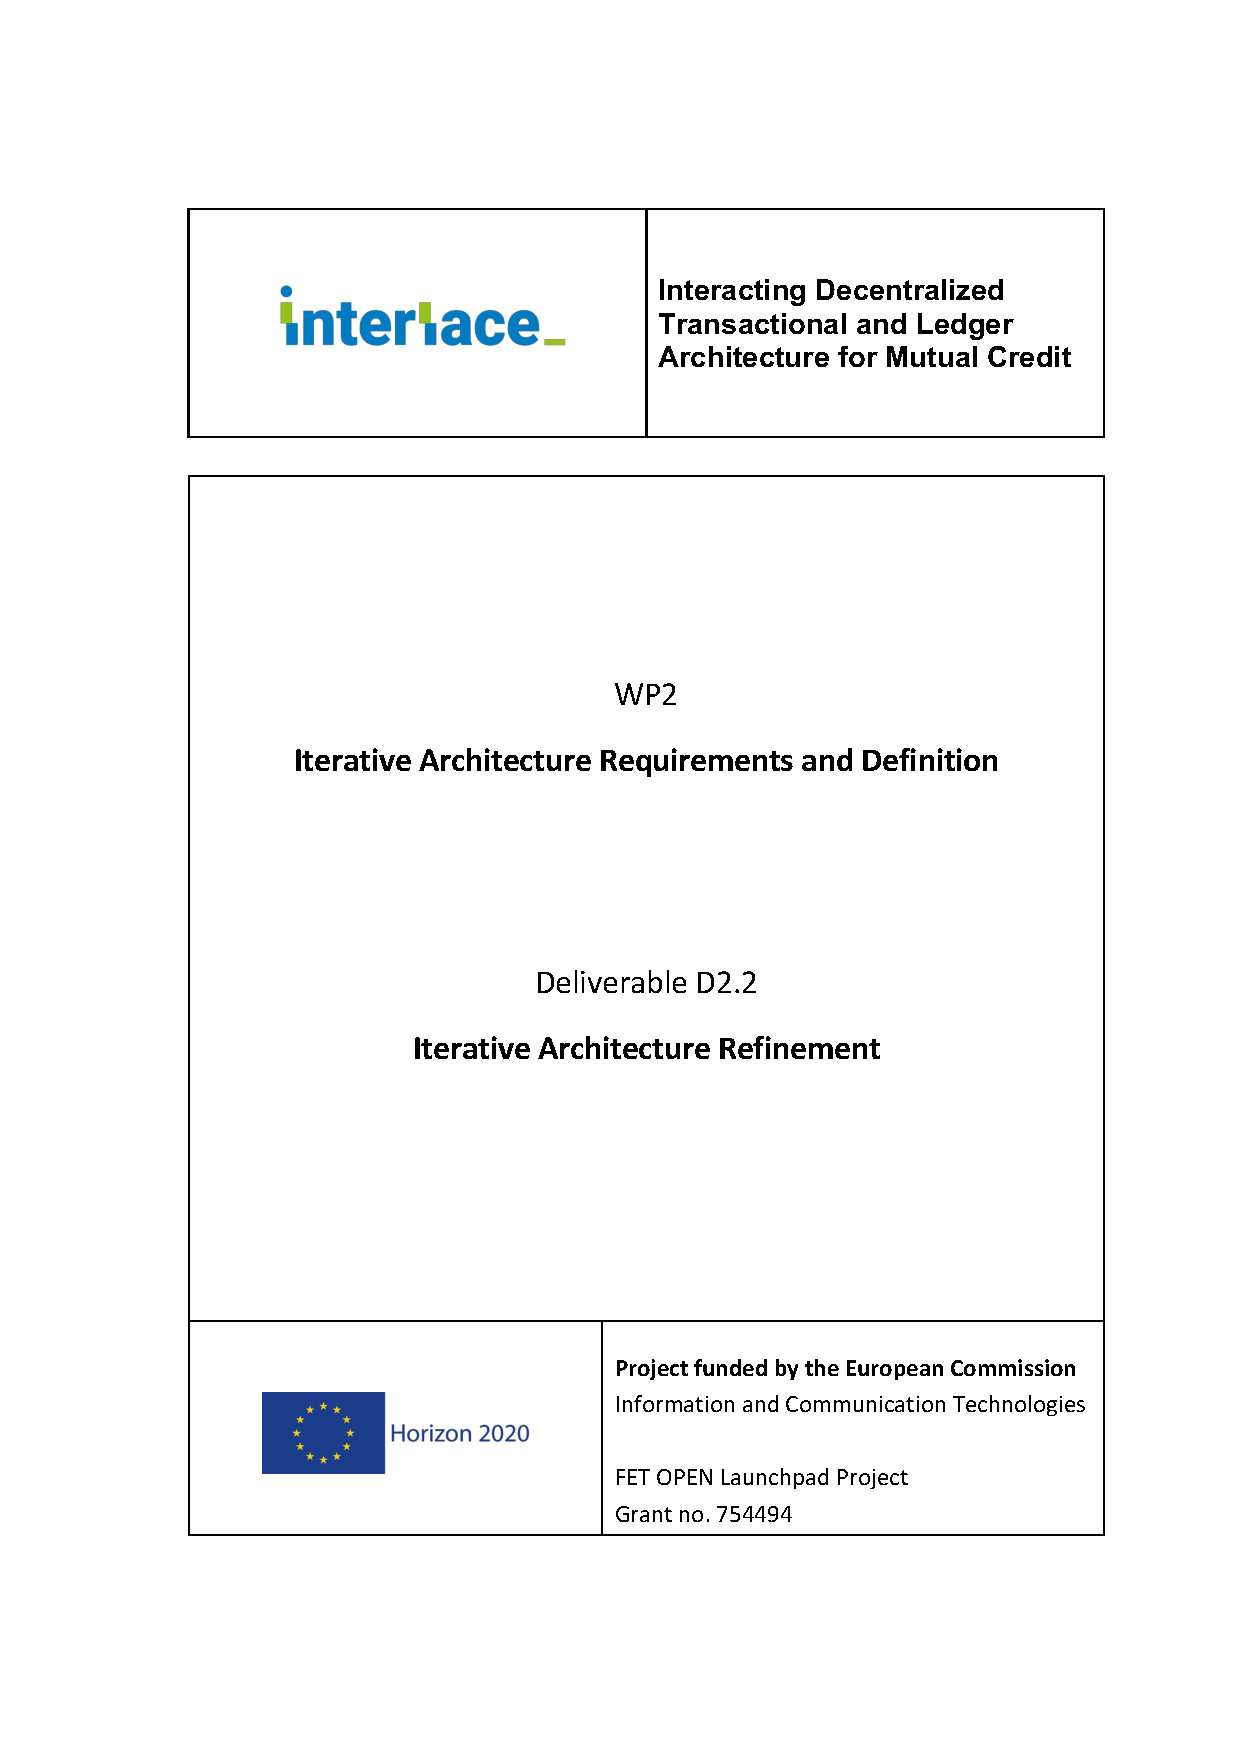
\includepdf[pages=-, scale=1.0]{Misc/Front}

%===================================================
%================== ABSTRACT
%===================================================
\thispagestyle{empty}

\begin{abstract}
\normalsize


\end{abstract}

\newpage

%===================================================
%================== TABLE OF CONTENTS
%===================================================
\tableofcontents

%===================================================
%================== CHAPTERS
%===================================================
\chapter{Introduction}
\label{ch:Introduction}

\vspace{-1cm}
\begin{center}
Paolo Dini and Giuseppe Littera
\end{center}

The selection of a blockchain technology for the INTERLACE platform has been a long and difficult process. The challenge has arisen from the wide variety of technologies, architectures, and protocols, from the very rapid rate of innovation in this field, and from the evolving requirements of a future vision for the Sardex platform. This is because, although INTERLACE is only a first attempt at a blockchain-based transactional platform for the Sardex circuit, it should be as compatible as possible with the future vision of the circuit.

The future vision of the Sardex circuit has been difficult to define because it took a long time to understand how the Sardex mutual credit system could scale to global level while remaining faithful to its principles of support for local economies and of reliance on trust between its users. Since the social and the business dimensions are the starting point for the requirements that lead to choice of technology and architecture definition, we adopted a circular and iterative approach that compared what was possible with what is desirable at each step, and slowly evolved the vision as our understanding of the blockchain space and of our own requirements improved. In this short report we cannot go into too much depth, but it is worth addressing what is arguably the central concept for both Sardex and the blockchain: trust.

\section{Sardex, Trust and the Blockchain}
The blockchain is often described as a `trustless' technology, since the distribution of the validation and record-keeping function to many independent nodes, together with cryptographic algorithms, removes the need for a central authority that plays the role of record keeper and transaction orderer. According to the prevailing view in Computer Science, therefore, trust in a central authority and bilateral trust between transacting parties are substituted for reliance on a type of technology and protocol. Clearly, such an approach is particularly useful in situations where there is not trust at all between transacting parties.

By contrast, the Sardex circuit relies on trust to a very significant extent. Between the ``sociological'' trust discussed by Sartori and Dini \cite{SartoriDini2016} and the trust in the technology platform lies an ``economic'' type of trust. In particular, Sardex relies on, and reinforces, ``thick trust''.\footnote{Richard Simmons, economist, private communication, 2018.} Thick trust has been discussed in the literature in the business context (e.g. \cite{VosselmanMeerKooistra2009}), but for our purposes it is sufficient to define it as the combination of ``Know Your Customer'' with ``Know Their Products''. The role of the Sardex company that runs the circuit, combined with the work of the Sardex brokers, greatly reduces the social cost of trust for the SMEs who participate in the network and achieves and combines both these components, because it is able to make trust transitive: the circuit members trust the Sardex company and the electronic platform, and in the majority of cases this trust extends to bilateral trust between the transacting parties, making the Sardex circuit a particularly strong and stable trading community.

One of the drawbacks of such an approach is that the communities and companies involved in the network ultimately depend on one actor to facilitate credit and trade among participants, rendering the network as a whole highly efficient yet vulnerable and not as inclusive and socially/financially adoptable as might be preferred.

Why, then, is Sardex interested in the blockchain? For two reasons. First, as the company operations grow beyond Sardinia and Italy to other countries in Europe and beyond they will involve interactions with other circuits whose legal personality, business relationship with Sardex, and proprietary structure may vary along a range of options depending on the context and stakeholders. Therefore, from a functional and organisational point of view it may be more expedient to build in some flexibility at the level of the architecture: for example, each circuit could run a separate node of the blockchain. This could enable inter-circuit trade via agreements recorded on distributed ledgers, more transparency of the overall network, and regional and local clusters of SMEs -- which in turn reduces informational asymmetries.

Second, this organisational flexibility requirement, which is essentially functionalist, is reinforced by the social and cultural requirement of respecting local community identity to the extent possible. This is not so much a matter of institutional or governance efficiency as a question of shared values built around reciprocal respect between different communities who identify with different regions or localities. We feel it is easier to meet such expectations with an articulated and decentralised\footnote{In contrast to what we wrote in the INTERLACE proposal, we have adopted the definition of `decentralised' as an architecture where control is distributed, as opposed to `distributed', which refers only to a distribution of functional aspects but leaves the control central.} architecture than through a monolithic platform like Facebook or Google.

\section{Overview of Report}
This brief report provides a high-level discussion of the main blockchain technologies we examined during the course of the project, together with a rationale for choosing Hyperledger as the core component with possible extensions towards Ethereum and Holochain. The discussion in the rest of the report assumes familiarity with the basic concepts and terminology of the main blockchain technologies as can be found, for example, in \cite{TascaEtAl2017}.

Chapter \ref{ch:dlt} discusses a few candidate Distributed Ledger Technologies (DLTs) that we assessed in the process of deciding which satisfied the INTERLACE and Sardex requirements best. The next step in the process was going to be an ASIM specification and CoreASIM modelling of the transactional platform, which would have been reported in a third chapter, but lack of funding complementary to INTERLACE made this plan impossible. We therefore decided that it made more sense to focus the remaining time and resources on implementing a proof-of-concept transactional platform based on the requirements specified in deliverable D2.1 \cite{INTERLACE_D21} and updated in deliverable D3.1 \cite{INTERLACE_D31}. The implementation work is reported in deliverable D3.2.



\section{Table of Acronyms}
Table \ref{acronyms} shows the definition of the acronyms used in this report.


\begin{table}
\begin{centering}
{\begin{tabular}{| r | c | l |}
\hline
AML		&& Anti Money Laundering\\
\hline
ASM		&& Abstract State Machine \\
\hline
ASIM	&& Abstract State Interaction Machine \\
\hline
B2B		&& Business-to-Business\\
\hline
B2C		&& Business-to-Consumer\\
\hline
BFT		&& Byzantine Fault Tolerance\\
\hline
BTC		&& Currency symbol for Bitcoin\\
\hline
Dapp	&& Distributed App\\
\hline
DB		&& Database\\
\hline
DHT		&& Distributed Hash Table\\
\hline
DLT		&& Distributed (or Decentralised) Ledger Technology\\
\hline
DoS		&& Denial of Service\\
\hline
ETH		&& Currency symbol for Ether, the Ethereum token\\
\hline
EVM		&& Ethereum Virtual Machine\\
\hline
FDAS	&& Federated Distributed Agreement System\\
\hline
FPML	&& Financial Products Markup Language\\
\hline
GDPR	&& General Data Protection Regulation\\
\hline
ICO		&& Initial Coin Offering\\
\hline
JS		&& Javascript\\
\hline
JVM		&& Java Virtual Machine\\
\hline
KYC		&& Know Your Customer\\
\hline
LE		&& Leader Election\\
\hline
PBFT	&& Plenum Byzantine Fault Tolerance\\
\hline
PoA		&& Proof of Authority\\
\hline
PoS		&& Proof of Stake \\
\hline
PoW		&& Proof of Work\\
\hline
QI		&& Quorum Intersection\\
\hline
REST 	&& Representational State Transfer\\
\hline
SC		&& Smart Contract\\
\hline
SCP		&& Stellar Consensus Protocol\\
\hline
SMR		&& State Machine Replication\\
\hline
SQL		&& Structured Query Language\\
\hline
SRD		&& Currency symbol for Sardex credits\\
\hline
Tx/s		&& Transactions per second\\
\hline
UML		&& Unified Modelling Language\\
\hline
UTXO	&& Unspent Transaction Output\\
\hline
XLM		&& Currency symbol for Lumen, the Stellar token\\
\hline
\end{tabular}}
\caption{\bf \small Table of acronyms used in the report}
\label{acronyms}
\end{centering}
\end{table}











\newpage












\chapter{Analysis of Possible Blockchain Technologies for INTERLACE}
\label{ch:dlt}

\vspace{-1cm}
\begin{center}
Paolo Dini, Giuseppe Littera, ...
\end{center}

\section{Introduction}
The INTERLACE team has looked at a number of blockchain technologies:
\begin{packed_item1}
\item Corda
\item Holochain
\item Stellar
\item Quorum (permissioned Ethereum)
\item Hyperledger Fabric
\end{packed_item1}
In this chapter we analyse and discuss them in turn, emphasising the algorithmic, architectural,  mathematical, or financial aspects that are most pertinent to INTERLACE. The frameworks that have made it into this short list are all interesting for one reason or another, and at different points each of them was seriously taken into consideration for adoption. The one that comes closest to the requirements of the Sardex mutual credit system is Hyperledger. Therefore, after presenting and discussing the others Hyperledger will be analysed and presented in more detail. This will then form the basis for Chapter \ref{ch:bchain}, the blockchain specification chapter.

\section{Stellar}
\subsection{Introduction}
In this section we provide a mathematical summary of the Stellar Consensus Protocol (SCP) \cite{Mazieres2016}. The presentation involves a sequence of definitions interspersed with theorems and their proofs. Understanding the theorems and their proofs is essential to understanding the Stellar system and the SCP. Therefore, although we follow Mazi\`eres's paper \cite{Mazieres2016} very closely, we provide more elementary explanations of the mathematical formulation, relying on figures and diagrams created ad hoc as needed.

SCP is based on a new decentralized agreement system, also defined and developed in \cite{Mazieres2016}, called Federated Byzantine Agreement System (FBAS). FBAS and SCP, together, provide an alternative to Bitcoin's Proof of Work (PoW) \cite{Antonopoulos2015} or Ethereum's Proof of Stake (PoS)\footnote{\url{https://github.com/ethereum/wiki/wiki/Proof-of-Stake-FAQ}} to achieve consensus. FBAS is a generalization of Byzantine agreement,\footnote{\url{https://en.wikipedia.org/wiki/Byzantine_fault_tolerance}} where the latter is analogous to a permissioned system. Although the early implementation of the new Sardex INTERLACE platform will be permissioned, we wish to develop an architecture that can easily replace centralized control with local consistency between transacting parties. At the level above in the network hierarchy, we will also need to manage a federated network of circuits. Also here the capability to transition to a scalable decentralized architecture is preferable to a traditional centralized approach, although at this level Corda may be a more appropriate Distributed Ledger Technology (DLT) framework.

\subsection{Federated Byzantine Agreement System}
\subsubsection{Basic Components\\}

A Stellar network relies on a FBAS to achieve consensus in the absence of central control. The consensus is on the update of replicated states such as ledger records corresponding to transactions. The purpose of the consensus protocol is for a set of nodes to reach agreement on a given update. Each update is identified with a unique \emph{slot} which also encodes information on inter-update dependencies -- for example as consecutively numbered positions in a transaction ledger. A FBAS runs a SCP that ensures that the nodes agree on slot contents. Agreement is defined in terms of safety of operation; the definition is somewhat recursive so it may need to be refined later:
\begin{defin}
We say that a node $v$ can \emph{\bf safely} apply update $x$ in slot $i$ when
\begin{packed_item1}
\item it has safely applied all the updates in all the slots upon which $i$ depends, and
\item it believes all correctly functioning nodes will eventually agree on $x$ for slot $i$.
\end{packed_item1}
\end{defin}
\smallskip
\begin{defin}
When node $v$ has safely applied update $x$ in slot $i$ we say that $v$ has \emph{\bf externalized} $x$ for slot $i$.
\end{defin}
The reason for this term is that once the contents of a slot have been accepted by other nodes they (the other nodes) could perform irreversible actions as a consequence, which $v$ cannot do anything about: the contents are now outside or \emph{external} to the control of the originator node $v$.

A challenge for FBA is that malicious nodes can outnumber honest ones, such that determining a quorum by simple majority is not sufficient to guarantee safety. FBA selects quorums in a decentralized way, leading to a layering of the network into a hierarchy such that different structures are relevant at different levels, as shown in Figure \ref{fig:vqQUV}. The top level is provided by a set of nodes $V$. The second level is called a `quorum', denoted by $U$ and defined as a set of nodes sufficient \emph{for those nodes} to reach agreement. The level below is a set of `slices' of a given node $v$, written $Q(v)$, where a slice is a subset of a quorum whose nodes agree with that \emph{single} node $v$. As the figure shows, a node $v$ may belong to more than one slice, with the cardinality of $Q(v)$ (i.e.\ $|Q(v)|$) providing the quantification. We now provide formal definitions and mathematical relations between these quantities.

\begin{figure}[h]
\centering
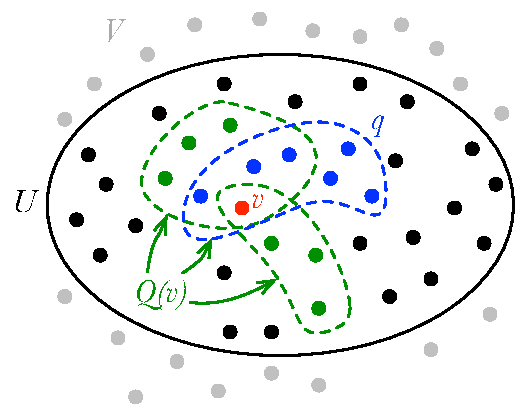
\includegraphics[width=8 cm]{Figures/vqQUV}
\caption{\bf \small The five levels of a Stellar network or FBAS}
\label{fig:vqQUV}
\end{figure}

Using the usual notation $2^X$ for the power set\footnote{The power set of a set $X$ is the set of all possible subsets of $X$ \cite{Cameron2008}. For a set of $N$ elements, its power set turns out to have $2^N$ elements, hence the notation.} of the set $X$, $2^V$ is the power set of $V$, i.e.\ the set of all possible quorum slices. At the next level, $2^{2^V}$ is the power set of quorum slices, i.e. the set of all possible \emph{sets} of quorum slices. Figure \ref{fig:SliceAndQ} shows a visualization of the elements of these kinds of power sets.

\begin{figure}[h]
\centering
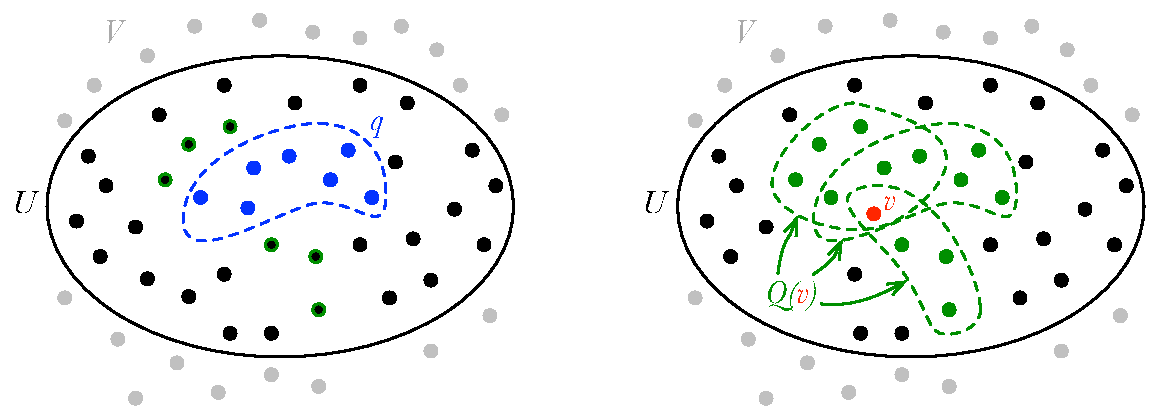
\includegraphics[width=15 cm]{Figures/SliceAndQ}
\caption{\bf \small LEFT: a) $q$ is an element of $2^V$. RIGHT: b) $Q(v)$ is an element of $2^{2^V}$.}
\label{fig:SliceAndQ}
\end{figure}

The function $Q$ assigns to each node $v \in V$ a set of slices $\{ q_1, q_2, \cdots, q_k \}$. Here the curly brackets denote set and $k$ is the number of slices for a given node $v$. Formally,
\begin{align}
Q\colon V \rightarrow 2^{2^V} \setminus \emptyset,
\end{align}
where $\setminus \emptyset$ means that the empty set is not in the range of this function ($Q(v)$ can never be empty).\footnote{It is not immediately clear whether this is a consequence of how this function operates or whether it is a requirement that we are adding arbitrarily to ensure that it does what we need. \textcolor{red}{TBD.}} In general,
\begin{align}
\forall v \in V, \forall q \in Q(v), \qquad v \in q,
\end{align}
which reads `For all nodes $v$ members of the set $V$ and for all slices $q$ members of the set $Q(v)$, node $v$ is a member of some slice $q$'.
\begin{defin}
A Federated Byzantine Agreement System \emph{(\textbf{FBAS})} is a pair $(V, Q)$.
\end{defin}
\begin{defin}
\label{quorum}
A set of nodes $U \subseteq V$ in a FBAS $(V, Q)$ is a \emph{\textbf{quorum}} iff $U \ne \emptyset$ and $U$ contains a slice for each member:
\begin{align}
\forall v \in U, \exists q \in Q(v) \ | \  q \subseteq U.
\end{align}
\end{defin}
In English: for all $v$ members of a quorum $U$, there exists a slice $q$, member of $Q(v)$, such that the slice is a subset of, or equal to, the quorum $U$. A quorum can also be described as a set of nodes sufficient to reach agreement.
\begin{defin}
\label{quorumslice}
A \emph{\textbf{quorum slice}} $q$ is a subset of a quorum $U$ sufficient to convince a particular node $v$ of agreement.
\end{defin}
Therefore, a quorum slice is usually smaller than a quorum, as shown in the figures above.

The `convincing' is depicted graphically by an arrow that indicates dependence between nodes in a manner analogous to inheritance in UML class diagrams. For example, as shown in Figure \ref{fig:convincing}a, $v_2$ can convince $v_1$ but not vice versa, i.e.\ $v_1$ depends on itself and on $v_2$ while $v_2$ depends only on itself. Figure \ref{fig:convincing}b shows the corresponding slices. Note that in this simple case the quorum of this set of nodes $V = \{ v_1, v_2 \}$ equals the slice for $v_1$: $V = U = q(v_1) = \{ v_1, v_2 \}$, whereas the set of slices $Q(v_1)$ is written $Q(v_1) = \{ \{ v_1, v_2 \} \}$, where the outer curly brackets indicate the set of slices $Q(v_1)$ and the inner curly brackets indicate the slice $q_1 = q(v_1)$.

\begin{figure}[h]
\centering
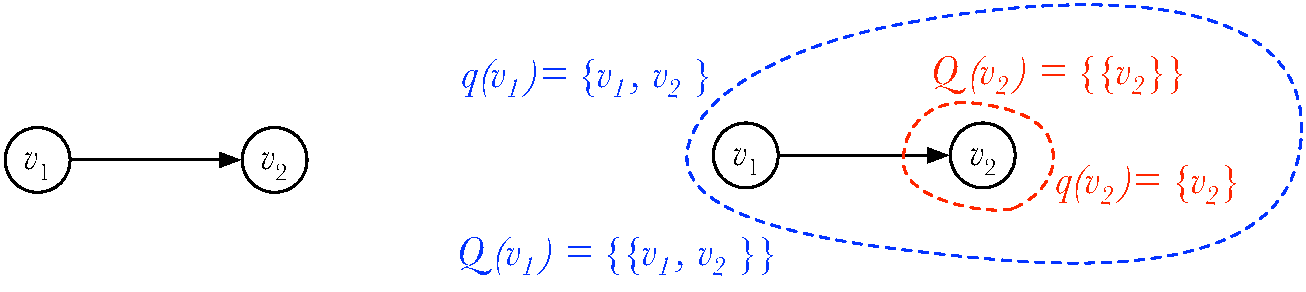
\includegraphics[width=15 cm]{Figures/convincing}
\caption{\bf \small LEFT: a) $v_2$ can convince $v_1$ but not vice versa. RIGHT: b) The slices of $v_1$ and of $v_2$.}
\label{fig:convincing}
\end{figure}

\subsubsection{Examples\\}
Figure \ref{fig:example1} shows a more complex interdependence between a set of 4 nodes, as Example 1. The arrows imply that $v_2$, $v_3$, and $v_4$ each has the same slice. Thus, $q(v_1) = q(v_2) = q(v_3) = \{ v_2, v_3, v_4 \}$. In this case we also have that $Q(v_2) = Q(v_3) = Q(v_4) = \{\{ v_2, v_3, v_4 \} \}$. In this example, although $\{\{ v_2, v_3, v_4 \} \}$ is a quorum, the smallest quorum involving $v_1$ must involve all four nodes.

\begin{figure}[h]
\centering
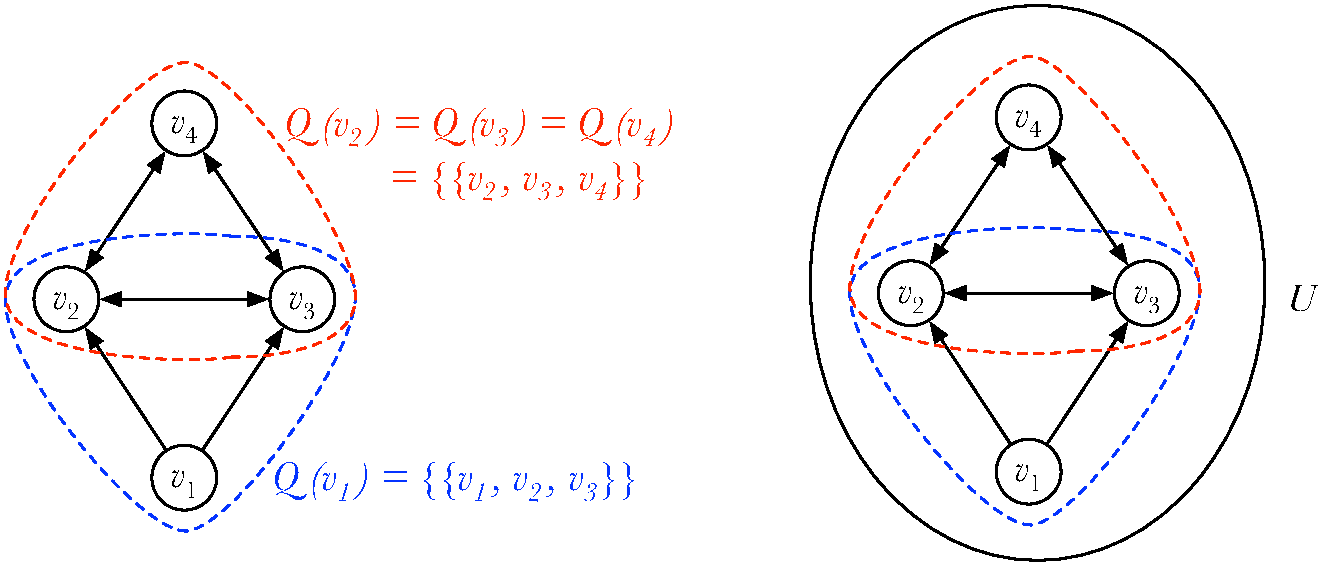
\includegraphics[width=15 cm]{Figures/example1}
\caption{\bf \small Example 1. L: a) The slices of this network. R: b) The smallest quorum involving $v_1$. (After \cite{Mazieres2016})}
\label{fig:example1}
\end{figure}

In traditional, non-federated Byzantine systems all nodes have the same slices. Therefore, non-federated systems do not distinguish between slices and quorums:
\begin{align}
\forall v_i, v_j \in V, \qquad Q(v_i) = Q(v_j). \qquad\qquad \text{[BAS]} 
\end{align}
In our case, instead, in general we have that
\begin{align}
\forall v_i, v_j \in V, \qquad Q(v_i) \ne Q(v_j). \qquad\qquad \text{[FBAS]} 
\end{align}
The important point made by Mazi\`eres is that whereas BAS is not scalable, as exemplified by the huge CPU overhead the Bitcoin consensus protocol requires, FBAS is scalable.

\begin{center}
\small
\frame{\colorbox{light-gray}{\makebox[16.5cm]{\parbox{16.5cm}{
%\vspace{.2cm}
\begin{quote}
\textbf{Example 2}

It is worth discussing a second example from Mazi\`eres, as shown in Figure \ref{fig:example2}. The figure shows three new notational concepts:
\vspace{.3cm}
\begin{packed_item1}
\item a reflexive dependence arrow can be drawn explicitly
\item sets of nodes can be grouped explicitly into separate sets or tiers, and
\item the dependence arrows can carry specific labels.
\end{packed_item1}
\end{quote}
\vspace{.2cm}
}}}}
\end{center}

\begin{center}
\small
\frame{\colorbox{light-gray}{\makebox[16.5cm]{\parbox{16.5cm}{
%\vspace{.2cm}
\begin{quote}
\vspace{.2cm}
For example, the label on the reflexive arrow on the top tier indicates that at least 3 nodes are needed for consensus. According to the definitions above for the arrow directions, the top tier does not depend on the tiers below, and it is precisely for this reason that it is the `top' tier. The label on the arrow between the middle and top tiers indicates that the slice of any one node from the middle tier is composed of itself plus any two of the tier above. The slice of either $v_9$ or $v_{10}$ is composed of itself plus any two nodes from the middle tier. Since each of these, in turn, depends on any two of the nodes of the top tier, the size of the slice will be at least 5 and at most 7 nodes.
\end{quote}
\vspace{-.5cm}
\begin{figure}[H]
\centering
\captionsetup{width=11cm}
\frame{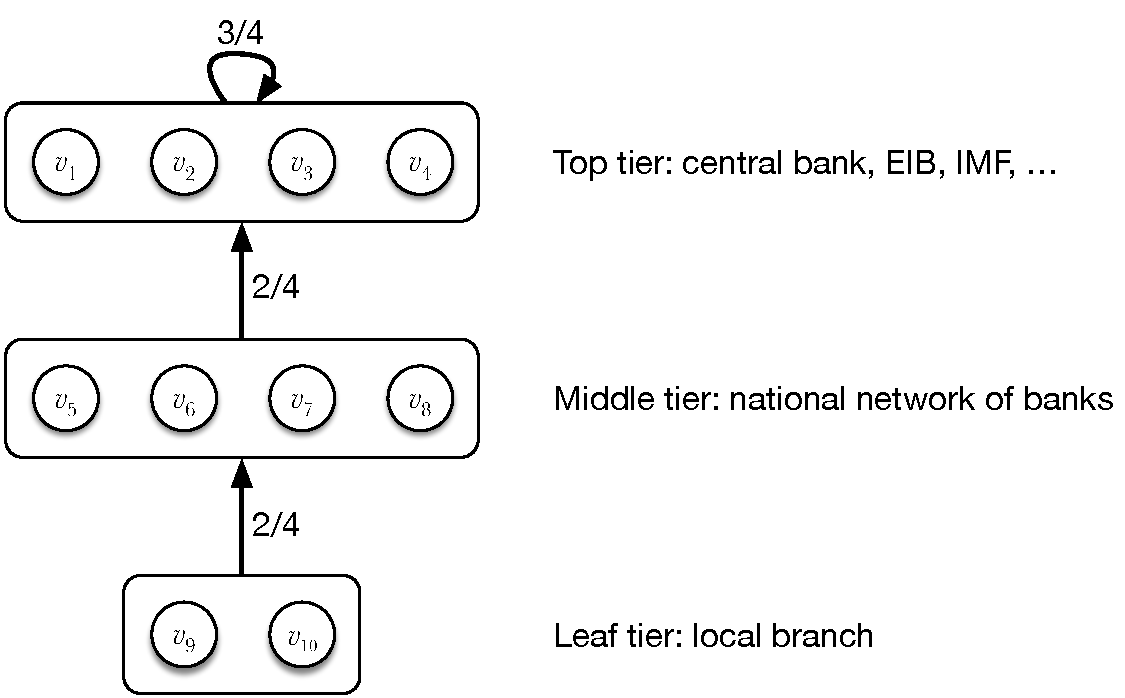
\includegraphics[width=11 cm]{Figures/example2}}
\caption{\bf \small Three-tier network (After \cite{Mazieres2016})}
\label{fig:example2}
\end{figure}

\begin{quote}
In Figure \ref{fig:example2} the top tier according to Mazi\`eres could be composed by a number of global financial institutions. The middle tier could be sets of banks operating at national level, with a single such set corresponding to a single country shown here. The bottom tier would be a single branch office, with the nodes inside representing individual customer accounts.
\end{quote}

\vspace{-.5cm}
\begin{figure}[H]
\centering
\captionsetup{width=15cm}
\frame{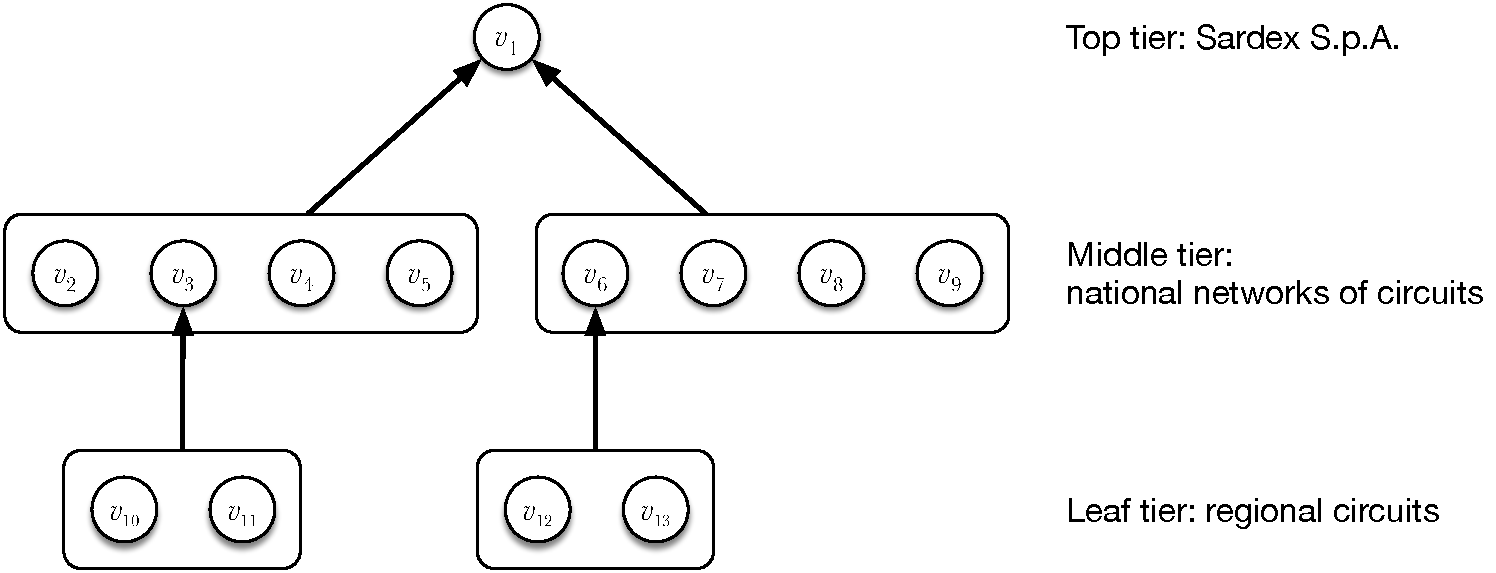
\includegraphics[width=15 cm]{Figures/example2_Sardex}}
\caption{\bf \small Possible mapping to INTERLACE circuit architecture. (After \cite{Mazieres2016})}
\label{fig:example2_Sardex}
\end{figure}

\begin{quote}
\vspace{-.3cm}
In Figure \ref{fig:example2_Sardex}, on the other hand, the top tier would be only the single Sardex S.p.A.\ company. The middle tier could be composed by different national jurisdictions, each of which containing a set of circuits; the figure shows two such jurisdictions corresponding to two different countries. The bottom tier would then correspond to separate individual circuits, with the nodes corresponding to individual company accounts. There are no labels on the arrows because the dependence is to a specific node in every case, generating a centralized hierarchical network.
\end{quote}
\vspace{.2cm}
}}}}
\end{center}

Although the architecture of Figure \ref{fig:example2_Sardex} may correspond to an initial implementation of the INTERLACE platform, it does not make use of the distribution capability of the Stellar consensus protocol, so let's proceed with the development of the protocol to see what will become possible.

\subsubsection{Safety and Liveness\\}
Nodes can be either well-behaved or ill-behaved. A well-behaved node chooses sensible quorum slices and obeys the protocol, including responding (eventually) to all requests. Ill-behaved nodes suffer Byzantine failure, meaning that they behave arbitrarily due for example to a malicious modification of the software, or may have crashed. The goal of FBAS is to ensure that all well-behaved nodes externalize the same values in spite of such ill-behaved nodes.

\begin{defin}
Two nodes in a set $V$ are \emph{\textbf{divergent}} if they externalize different values to the same slot. A set $V$ of nodes in a FBAS is \emph{\textbf{safe}} if no two of its elements (nodes) externalize different values for the same slot.
\end{defin}
\begin{defin}
A node $v \in V$ is \emph{\textbf{blocked}} if it is in some dead-end state from which consensus is no longer possible. A node $v \in FBAS$ has \emph{\textbf{liveness}} if it can externalize new values without the participation of any failed or ill-behaved nodes.
\end{defin}
\begin{defin}
Nodes that enjoy both safety and liveness are called \emph{\textbf{correct}}. Nodes that are not correct have \emph{\textbf{failed}}.
\end{defin}
Thus, nodes without liveness are blocked, whereas nodes without safety are divergent. Figure \ref{fig:correct} shows the set inclusion relationships between these different kinds of nodes in a set $V$. The reason a divergent or blocked node is shown under the well-behaved category even though it has failed is that, unlike ill-behaved nodes, it may have started as a correct node but may fail if its choice of slice causes it to wait indefinitely for messages from an ill-behaved node (this makes it {\bf blocked}) or, worse, if its state is maliciously modified by messages from an ill-behaved node (this makes it {\bf divergent}). Thus, the reason divergent nodes are a subset of the blocked nodes is that an attack that violates safety is strictly more powerful that one that violates only liveness.

\begin{figure}[h]
\centering
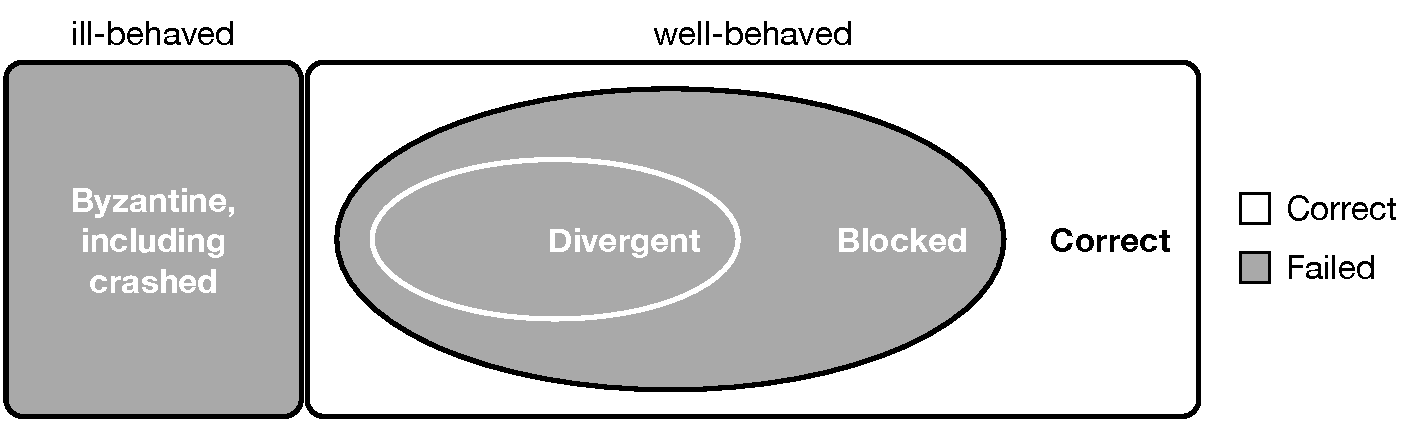
\includegraphics[width=14 cm]{Figures/correct}
\caption{\bf \small Set inclusion relationships between node categories. (After \cite{Mazieres2016})}
\label{fig:correct}
\end{figure}

Mazi\`eres explains that the above definition of liveness is weak because it only says that a node \emph{can} externalize, not that it \emph{will} or \emph{must}. As a consequence, there is a possibility for consensus to be forever delayed by, for example, preemptive reordering of the transactions. It is not clear whether this issue matters in the case of INTERLACE since we will not implement a completely decentralized system: some level of centralized control is likely to remain. Mazi\`eres in any case provides relevant references that can be consulted if this issue needs to be analysed in depth and resolved in some robust way.

\subsubsection{Optimal Resilience: Quorum Intersection and Dispensable Sets\\}
As is commonly assumed for asynchronous systems, messages between well-behaved nodes are eventually delivered, but can otherwise be delayed indefinitely or reordered arbitrarily. This section starts becoming more involved because it addresses the following non-trivial question: Given a specific $(V, Q)$ and a subset of $V$ that is ill-behaved, what are the best levels of safety and liveness that a FBAS can guarantee in an arbitrary network?

\smallskip
\begin{defin}
A FBAS has \emph{\textbf{quorum intersection}} iff any two of its quorums share at least one node.\footnote{The term `iff' means `if and only if'. It implies that the causal dependence works in both directions, in contrast to merely `if' which works only in the reverse direction. In symbols, `A iff B' is written $A \Leftrightarrow B$, whereas `A if B' is written $B \Rightarrow A$ and is also read as `B implies A'.} In other words, $\forall U_i, U_j \in FBAS, U_i \cap U_j \ne 0$, where $i$ and $j$ range over the number of quorums for a given FBAS.
\end{defin}

Therefore, when a FBAS has many quorums, quorum intersection (QI) fails when \textbf{\textit{any two}} do not intersect. We remind the reader that $Q(v_i)$ is just the set of slices of a given node $v_i$ and, depending on the slices of all the other nodes $v_j \in Q(v_i)$, may or may not be a quorum $U \subseteq V$. Thus, although in the simple examples that follow each $Q(v)$ is a quorum, this is by no means the case in general.

\begin{figure}[h]
\centering
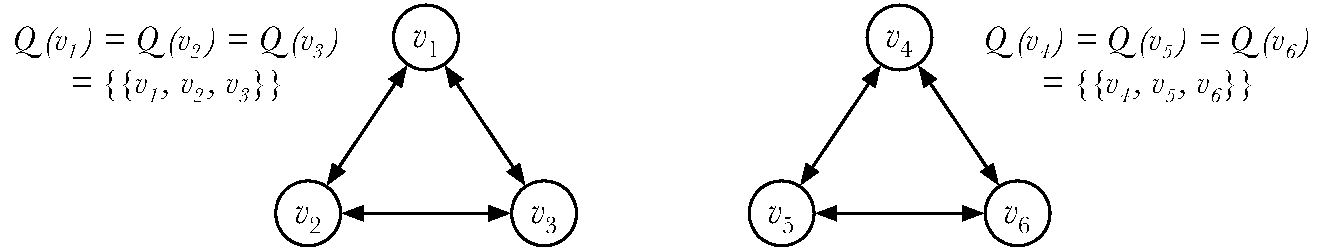
\includegraphics[width=15 cm]{Figures/QI1}
\caption{\bf \small A set of nodes without QI. (After \cite{Mazieres2016})}
\label{fig:QI1}
\end{figure}

Figure \ref{fig:QI1} shows a system of 6 nodes that lacks QI, since the function $Q$ allows two quorums on the set of 6 nodes that do not intersect. Mazi\`eres says that the two quorums can separately agree on contradictory statements, which makes sense at an abstract level but not so much in the case of this example. In other words, if $v_5$ cannot communicate with $v_1$ how can it say something about $v_1$ that $v_1$ might not agree with? We will not have a satisfactory answer until we know more about what different nodes can say about each other, and how. In the meantime, what Mazi\`eres says is partly helpful. Namely, he says that the whole set of all nodes $\{ v_1, \cdots, v_6 \}$ is \emph{also} a quorum, which in this case we can call $U$, and it intersects the other two. Is this true? If we look back at the definition of a quorum (Definition \ref{quorum}), we can verify that yes, it is correct because each node has a slice that is part of $U$. So this is an example of a system that has multiple quorums but two of them do not intersect and, therefore, the system does not have QI. We can believe that there is no certainty that $v_1$ can contradict or agree with $v_5$ even though they both belong to $U$.

\begin{figure}[h]
\centering
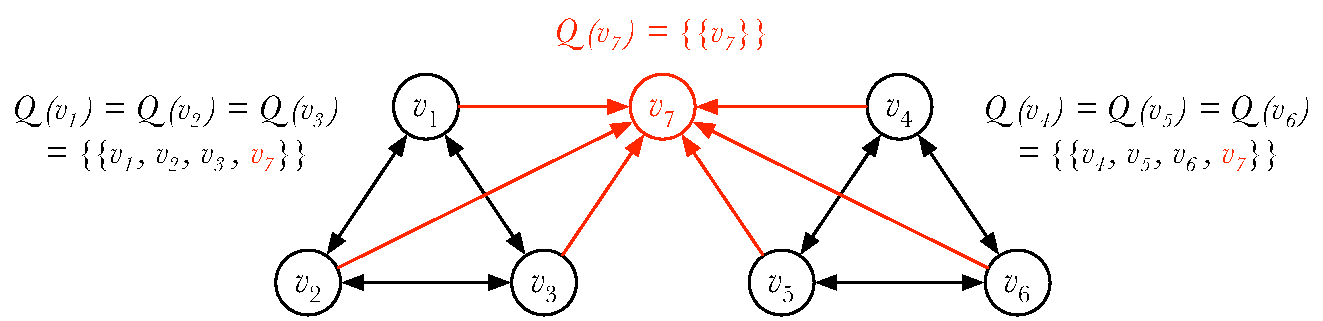
\includegraphics[width=15 cm]{Figures/QI2}
\caption{\bf \small A set of nodes with QI. (After \cite{Mazieres2016})}
\label{fig:QI2}
\end{figure}

Safety cannot be guaranteed because such a system can operate like two separate FBAS systems that do not communicate. However, safety may not be possible even in a system with QI, like the one shown in Figure \ref{fig:QI2}, if the intersecting node is ill-behaved. If $v_7$ makes inconsistent statements to the left and right quorums they are as good as disconnected. Therefore, safety can be guaranteed only if the well-behaved nodes have QI; or, put otherwise, a FBAS $(V, Q)$ can survive Byzantine failure by a set $B \subseteq V$ iff $(V, Q)$ has QI after deleting the nodes in $B$ from $V$ and from all slices in $Q$. 

More formally,
\begin{defin}
If $(V, Q)$ is a FBAS and $B \subseteq V$ is a set of nodes, then to \emph{\textbf{delete}} $B$ from $(V, Q)$, written $(V, Q)^B$, means to compute the modified $(V \setminus B, Q^B)$, where
\begin{align}
Q^B(v) = \{ q \setminus B\ |\ q \in Q(v) \},		\qquad \forall v \in V \setminus B.
\end{align}
\end{defin}
It is the responsibility of each node $v$ to ensure that $Q(v)$ does not violate QI. From Mazi\`eress paper it is not clear {\bf how}, however. Be that as it may, assume that Figure \ref{fig:QI2} evolved from the 3-node FBAS $\{ v_1, v_2, v_3 \}$ to a system that includes also $\{ v_4, v_5, v_6 \}$. Assume now that $\{ v_4, v_5, v_6 \}$ are malicious such that they choose slices that do not satisfy QI. But $Q(v)$ is meaningless for a malicious node. That's why the necessary condition for safety, QI after deleting ill-behaved nodes, is unaffected by the slices of ill-behaved nodes. The system $(V, Q)^{ \{ v_4, v_5, v_6 \} }$ restores QI for $\{ v_1, v_2, v_3 \}$. Note that we have not yet said how such deletion takes place. For now we just say that the protocol must guarantee safety for $\{ v_1, v_2, v_3 \}$ without these nodes having to know that $\{ v_4, v_5, v_6 \}$ are malicious.

Turning now to dispensable sets or DSets, the safety and liveness of the nodes outside a DSet can  be guaranteed regardless of the behaviour of the nodes inside the DSet.
\begin{defin}
Let $(V, Q)$ be a FBAS and $B \subseteq V$ be a set of nodes. We say that $B$ is a dispensable set or a \emph{\textbf{DSet}} iff:
\begin{packed_item1}
\item $(V, Q)^B$ has QI \qquad\qquad\qquad\qquad\ (Intersection)
\item $V \setminus B$ is a quorum OR $B = V$ \qquad (Availability)
\end{packed_item1}
\end{defin}
As explained by Mazi\`eres, availability protects against nodes in $B$ not replying to requests or impeding other nodes' progress. QI protects against nodes in $B$ making contradictory assertions that enable other nodes to externalize inconsistent values for the same slot. These two threats depend on slice size in opposite ways: greater slices increase the chance for QI, but also the chance that they will contain failed nodes, impacting availability. Smaller slices decrease the chance of failed nodes, but also the likelihood of having QI.

The smallest DSet containing all ill-behaved nodes may contain also well-behaved nodes as well, if they depend on the ill-behaved ones. For example, in Figure \ref{fig:example2} if $v_5$ and $v_6$ are ill-behaved the smallest DSet would need to include also $v_9$ and $v_{10}$ since the lowest tier depends on any 2 of the nodes in the middle tier, and so it may depend on the two that are ill-behaved.

\begin{defin}
\label{intact}
A node $v \in FBAS$ is \emph{\textbf{intact}} iff $\exists\  DSET\  B$ containing all ill-behaved nodes and such that $v \notin B$.
\end{defin}

\begin{defin}
\label{befouled}
A node $v \in FBAS$ is \emph{\textbf{befouled}} iff it is not intact.
\end{defin}

\begin{theorem}
\label{theorem1}
Let $U$ be a quorum in FBAS $(V, Q)$, let $B \subseteq V$, and let $U' = U \setminus B$. If $U' \neq \emptyset$, then $U'$ is a quorum in $(V, Q)^B$.
\end{theorem}
\begin{proof}
First, since $U$ is a quorum, every $v \in U$ has a slice $q \in Q(v)$ such that $q \in U$:
\begin{align}
\exists q \in Q(v) | q\in U, \qquad \forall v \in U.
\end{align}
Second, since $U' \subseteq U$, every $v \in U'$ has $q \in Q(v)$ such that $q \setminus B \subseteq U'$:
\begin{align}
\exists q \in Q^B(v) | q \in U', \qquad \forall v \in U'.
\end{align}
Therefore, $U'$ is a quorum in $(V, Q)^B$.
\end{proof}
















\chapter{High-Level Hyperledger Architecture}
\label{ch:hl}

\vspace{-1cm}
\begin{center}
Paolo Dini, Giuseppe Littera, Eduard Hirsch and Luca Carboni
\end{center}

\section{Introduction}






\begin{figure}[h]
\centering
\frame{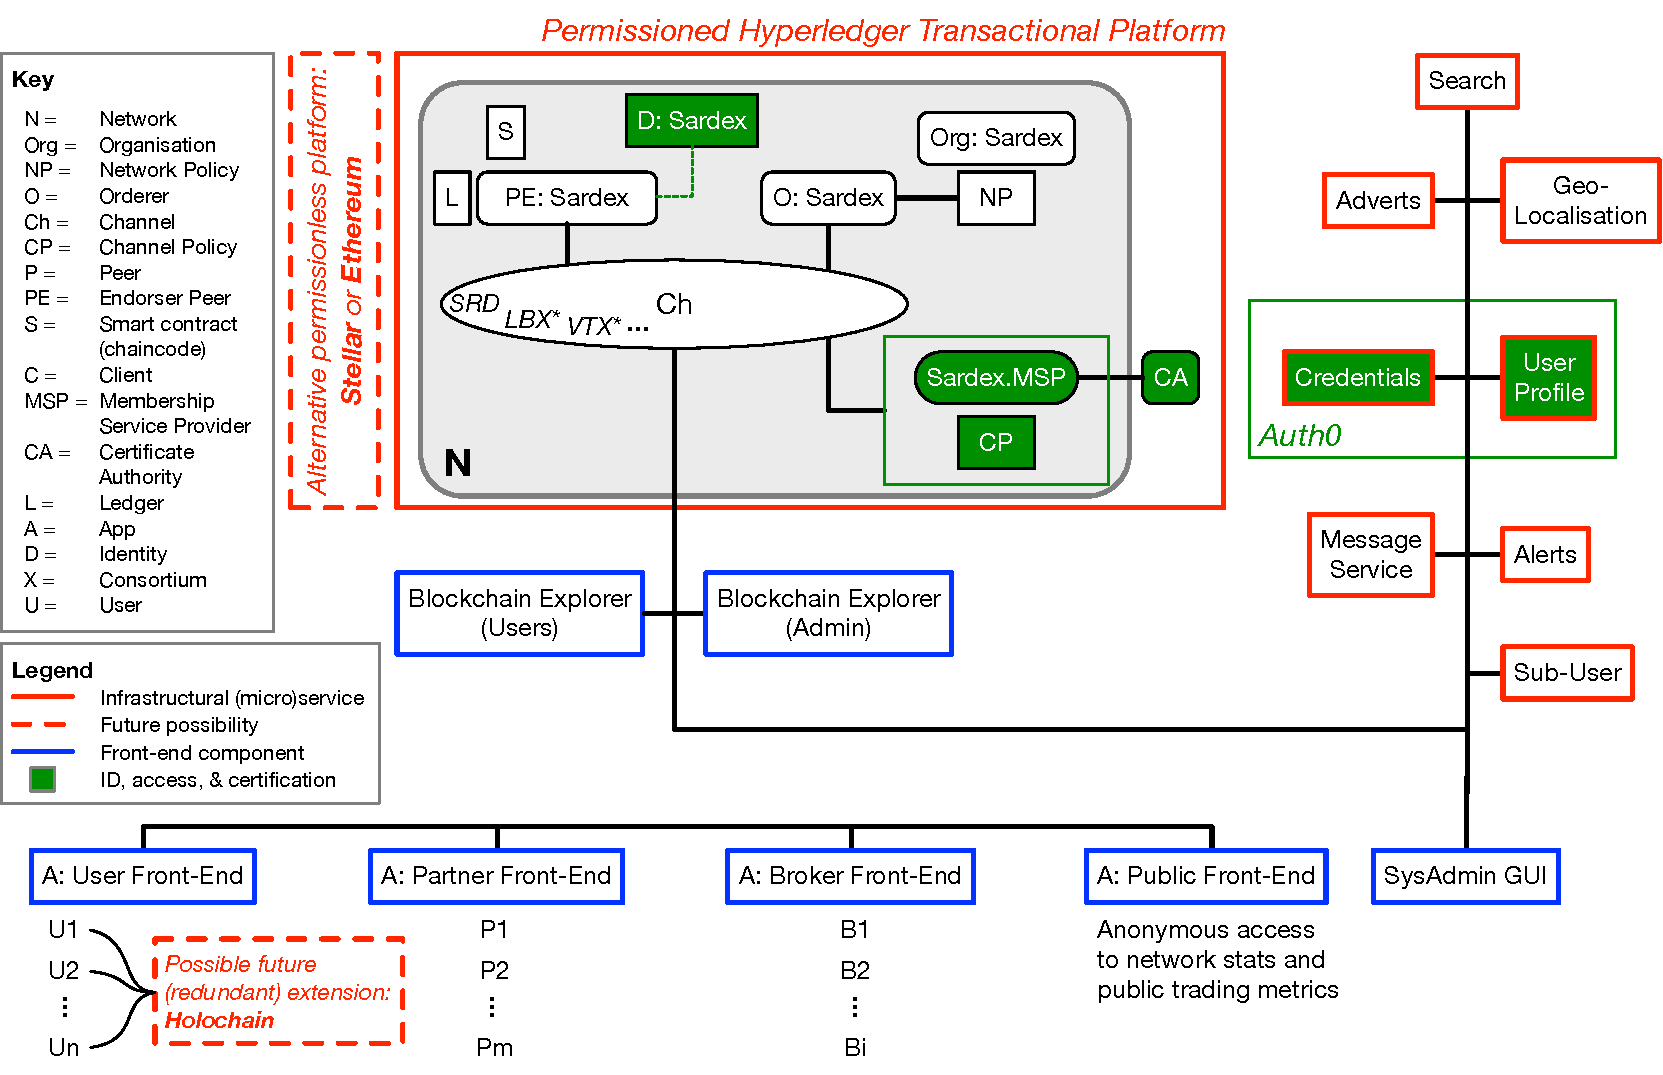
\includegraphics[width=16 cm]{Figures/HL_Architecture}}
\caption{\bf \small High-level Hyperledger-based microservice architecture with possible extensions}
\label{fig:HL_Architecture}
\end{figure}



\begin{figure}[h]
\centering
\frame{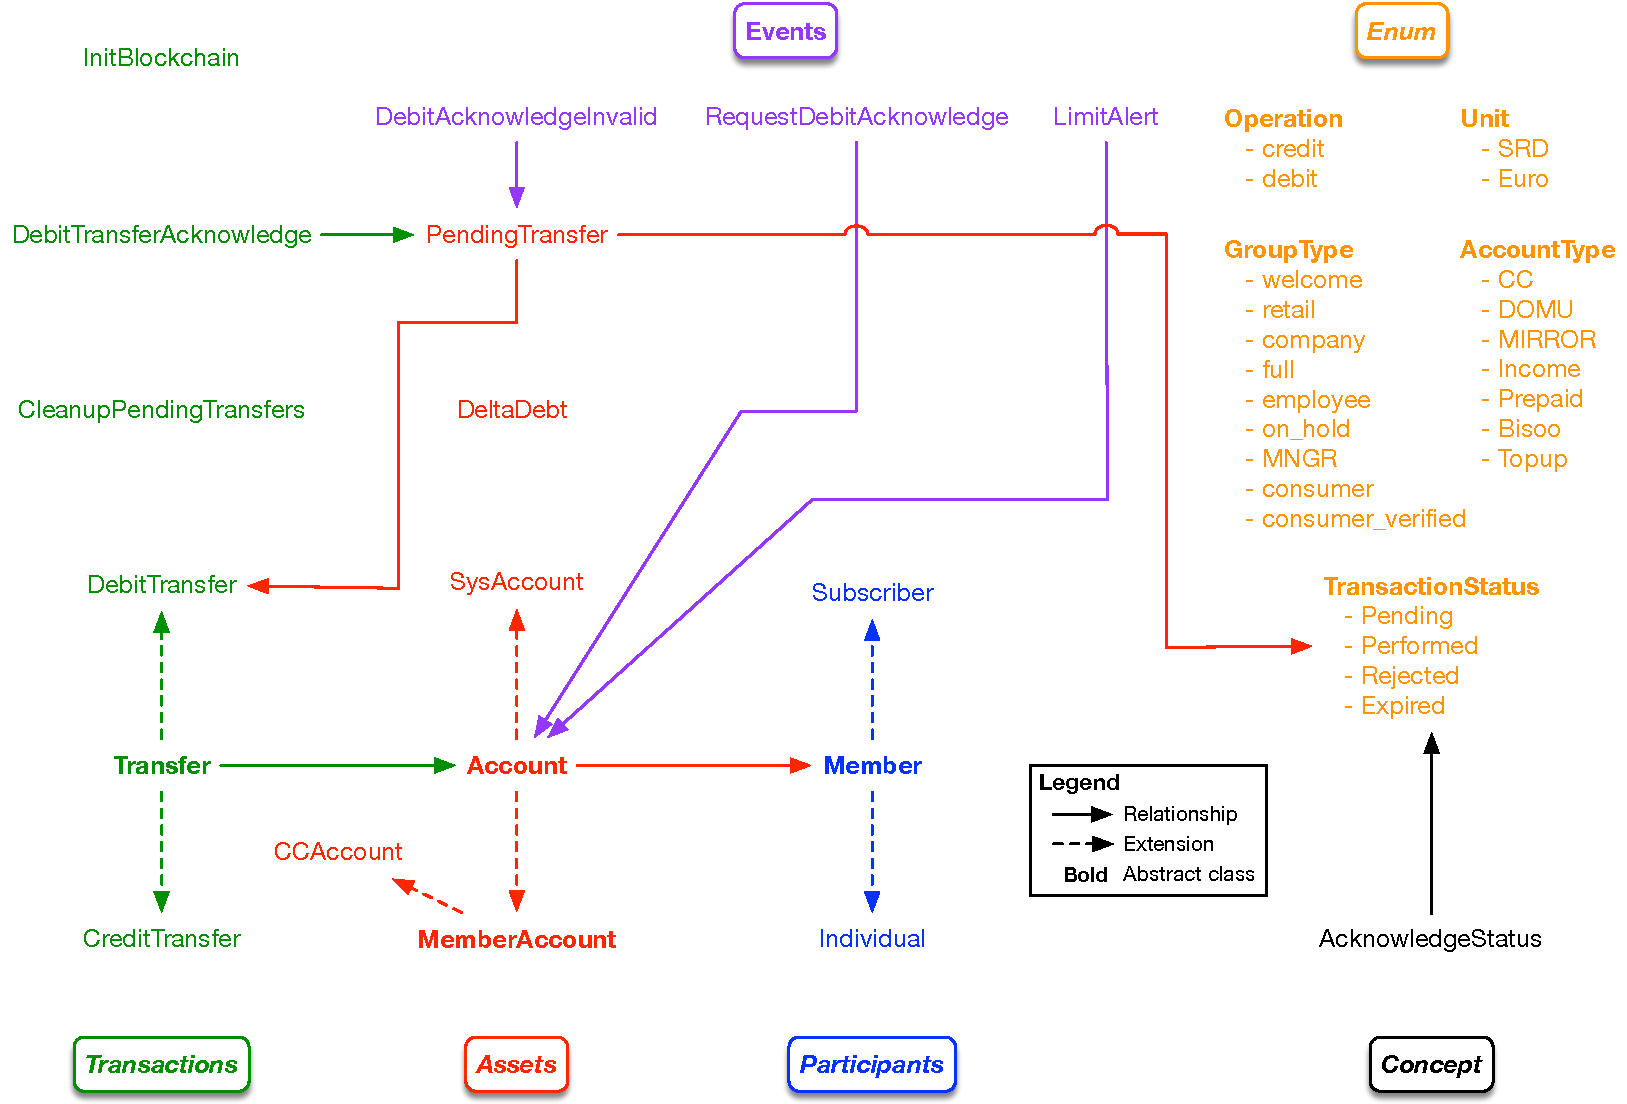
\includegraphics[width=16 cm]{Figures/DCN}}
\caption{\bf \small Hyperledger cto model/class diagram of transactional platform}
\label{fig:DCN}
\end{figure}








\chapter*{References}

\setlength{\parskip}{0.8\baselineskip}
\bibliographystyle{plainurl}
\small
\addcontentsline{toc}{chapter}{References}
\bibliography{Bib/BioComp_References}

%===================================================
%================== APPENDIX
%===================================================
\appendix
\addcontentsline{toc}{chapter}{Appendix: Basic Mathematical Framework for Stellar}
\setcounter{chapter}{1}
\renewcommand\thechapter{}
\makeatletter
\renewcommand\thesection{\@Alph\c@chapter.\@arabic\c@section}
\makeatother
\chapter*{Basic Mathematical Framework for Stellar}
\label{ch:stellar}

\vspace{-1cm}
\begin{center}
Paolo Dini
\end{center}

\section{Introduction}
In this Appendix we provide a mathematical summary of the Stellar Consensus Protocol (SCP) \cite{Mazieres2016}. The presentation involves a sequence of definitions interspersed with theorems and their proofs. Understanding the theorems and their proofs is essential to understanding the Stellar system and the SCP. Therefore, although we follow Mazi\`eres's paper \cite{Mazieres2016} very closely, in some cases we provide more elementary explanations of the mathematical formulation, relying on figures and diagrams created ad hoc as needed.

SCP is based on a new decentralized agreement system, also defined and developed in \cite{Mazieres2016}, called Federated Byzantine Agreement System (FBAS). FBAS and SCP, together, provide an alternative to Bitcoin's Proof of Work (PoW) \cite{Antonopoulos2015} or Ethereum's Proof of Stake (PoS)\footnote{\url{https://github.com/ethereum/wiki/wiki/Proof-of-Stake-FAQ}} to achieve consensus. FBAS is a generalization of Byzantine agreement,\footnote{\url{https://en.wikipedia.org/wiki/Byzantine_fault_tolerance}} where the latter is analogous to a permissioned system. Although the early implementation of the new Sardex INTERLACE platform will be permissioned, we wish to develop an architecture that can easily replace centralized control with local consistency between transacting parties. At the level above in the network hierarchy, we will also need to manage a federated network of circuits. Also here the capability to transition to a scalable decentralized architecture is preferable to a traditional centralized approach, although at this level Corda may be a more appropriate Distributed Ledger Technology (DLT) framework.

\section{Federated Byzantine Agreement System}
\subsection{Basic Components}

A Stellar network relies on a FBAS to achieve consensus in the absence of central control. The consensus is on the update of replicated states such as ledger records corresponding to transactions. The purpose of the consensus protocol is for a set of nodes to reach agreement on a given update. Each update is identified with a unique \emph{slot} which also encodes information on inter-update dependencies -- for example as consecutively numbered positions in a transaction ledger. A FBAS runs a SCP that ensures that the nodes agree on slot contents. Agreement is defined in terms of safety of operation; the definition is somewhat recursive so it may need to be refined later:
\begin{quote}
\vspace{-0.8cm}
\small
\begin{defin}
We say that a node $v$ can \emph{\bf safely} apply update $x$ in slot $i$ when
\begin{packed_item1}
\item it has safely applied all the updates in all the slots upon which $i$ depends, and
\item it believes all correctly functioning nodes will eventually agree on $x$ for slot $i$.
\end{packed_item1}
\end{defin}
\smallskip
\begin{defin}
When node $v$ has safely applied update $x$ in slot $i$ we say that $v$ has \emph{\bf externalized} $x$ for slot $i$.
\end{defin}
\end{quote}
The reason for this term is that once the contents of a slot have been accepted by other nodes they (the other nodes) could perform irreversible actions as a consequence, which $v$ cannot do anything about: the contents are now outside or \emph{external} to the control of the originator node $v$.

A challenge for FBA is that malicious nodes can outnumber honest ones, such that determining a quorum by simple majority is not sufficient to guarantee safety. FBA selects quorums in a decentralized way, leading to a layering of the network into a hierarchy such that different structures are relevant at different levels, as shown in Figure \ref{fig:vqQUV}. The top level is provided by a set of nodes $V$. The second level is called a `quorum', denoted by $U$ and defined as a set of nodes sufficient \emph{for those nodes} to reach agreement. The level below is a set of `slices' of a given node $v$, written $Q(v)$, where a {\bf slice} is a subset of a quorum whose nodes agree with that \emph{single} node $v$. As the figure shows, a node $v$ may belong to more than one slice, with the cardinality of $Q(v)$ (i.e.\ $|Q(v)|$) providing the quantification. We now provide formal definitions and mathematical relations between these quantities.

\begin{figure}[h]
\centering
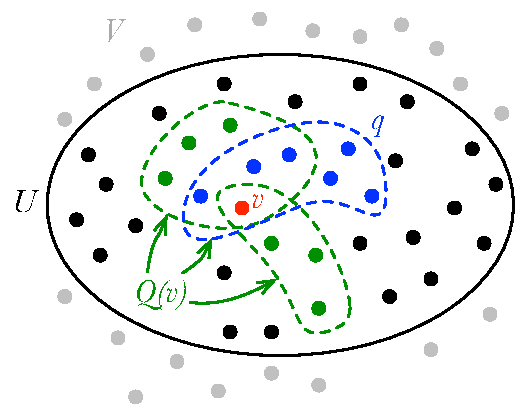
\includegraphics[width=7 cm]{Figures/vqQUV}
\caption{\bf \small The five levels of a Stellar network or FBAS}
\label{fig:vqQUV}
\end{figure}

Using the usual notation $2^X$ for the power set\footnote{The power set of a set $X$ is the set of all possible subsets of $X$ \cite{Cameron2008}. For a set of $N$ elements, its power set turns out to have $2^N$ elements, hence the notation.} of the set $X$, $2^V$ is the power set of $V$, i.e.\ the set of all possible quorum slices. At the next level, $2^{2^V}$ is the power set of quorum slices, i.e. the set of all possible \emph{sets} of quorum slices. Figure \ref{fig:SliceAndQ} shows a visualization of the elements of these kinds of power sets.

\begin{figure}[h]
\centering
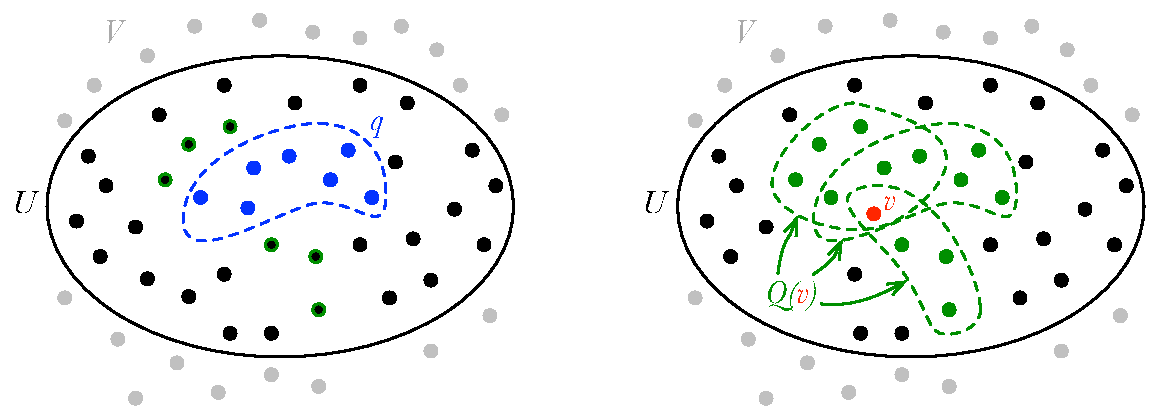
\includegraphics[width=15 cm]{Figures/SliceAndQ}
\caption{\bf \small L: a) $q$ is an element of $2^V$. R: b) $Q(v)$ is an element of $2^{2^V}$.}
\label{fig:SliceAndQ}
\end{figure}

The function $Q$ assigns to each node $v \in V$ a set of slices $\{ q_1, q_2, \cdots, q_k \}$. Here the curly brackets denote set and $k$ is the number of slices for a given node $v$. Formally,
\begin{align}
Q\colon V \rightarrow 2^{2^V} \setminus \emptyset,
\end{align}
where $\setminus \emptyset$ means that the empty set is not in the range of this function ($Q(v)$ can never be empty).\footnote{It is not immediately clear whether this is a consequence of how this function operates or whether it is a requirement that we are adding arbitrarily to ensure that it does what we need. \textcolor{red}{TBD.}} In general,
\begin{align}
\forall v \in V, \forall q \in Q(v), \qquad v \in q,
\end{align}
which reads `For all nodes $v$ members of the set $V$ and for all slices $q$ members of the set $Q(v)$, node $v$ is a member of some slice $q$'.
\begin{quote}
\vspace{-0.6cm}
\small
\begin{defin}
A Federated Byzantine Agreement System \emph{(\textbf{FBAS})} is a pair $(V, Q)$.
\end{defin}
\begin{defin}
\label{quorum}
A set of nodes $U \subseteq V$ in a FBAS $(V, Q)$ is a \emph{\textbf{quorum}} iff $U \ne \emptyset$ and $U$ contains a slice for each member:
\begin{align}
\forall v \in U, \exists q \in Q(v) \ | \  q \subseteq U.
\end{align}
\end{defin}
In English: for all $v$ members of a quorum $U$, there exists a slice $q$, member of $Q(v)$, such that the slice is a subset of, or equal to, the quorum $U$.
\begin{defin}
\label{quorumslice}
A \emph{\textbf{quorum slice}} $q$ is a subset of a quorum $U$ sufficient to convince a particular node $v$ of agreement.
\end{defin}
\end{quote}
Therefore, a quorum slice is usually smaller than a quorum, as shown in the figures above.

The `convincing' is depicted graphically by an arrow that indicates dependence between nodes in a manner analogous to inheritance in UML class diagrams. For example, as shown in Figure \ref{fig:convincing}a, $v_2$ can convince $v_1$ but not vice versa, i.e.\ $v_1$ depends on itself and on $v_2$ while $v_2$ depends only on itself. Figure \ref{fig:convincing}b shows the corresponding slices. Note that in this simple case the quorum of this set of nodes $V = \{ v_1, v_2 \}$ equals the slice for $v_1$: $V = U = q(v_1) = \{ v_1, v_2 \}$, whereas the set of slices $Q(v_1)$ is written $Q(v_1) = \{ \{ v_1, v_2 \} \}$, where the outer curly brackets indicate the set of slices $Q(v_1)$ and the inner curly brackets indicate the slice $q_1 = q(v_1)$.

\subsection{Examples}
Figure \ref{fig:example1} shows a more complex interdependence between a set of 4 nodes, as Example 1. The arrows imply that $v_2$, $v_3$, and $v_4$ each has the same slice. Thus, $q(v_2) = q(v_3) = q(v_4) = \{ v_2, v_3, v_4 \}$. In this case we also have that $Q(v_2) = Q(v_3) = Q(v_4) = \{\{ v_2, v_3, v_4 \} \}$. In this example, although $\{\{ v_2, v_3, v_4 \} \}$ is a quorum, the smallest quorum involving $v_1$ must involve all four nodes.

\begin{figure}[H]
\centering
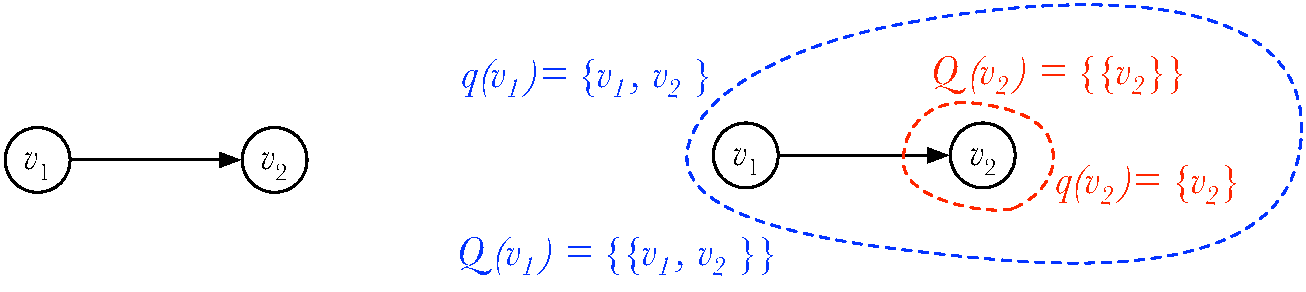
\includegraphics[width=15 cm]{Figures/convincing}
\caption{\bf \small L: a) $v_2$ can convince $v_1$ but not vice versa. R: b) The slices of $v_1$ and of $v_2$.}
\label{fig:convincing}
\end{figure}

Figure \ref{fig:example1} also provides a clear example of the difference between a slice and a quorum. The slice of $v_1$ is $q(v_1) = \{ v_1, v_2, v_3 \}$, which means that these three nodes are all that's needed to convince $v_1$. However, this set of nodes cannot be a quorum because the slices of $v_2$ and $v_3$ include nodes (actually only one node, $v_4$) that are outside of this set, which contravenes Definition \ref{quorum}.

\begin{figure}[h]
\centering
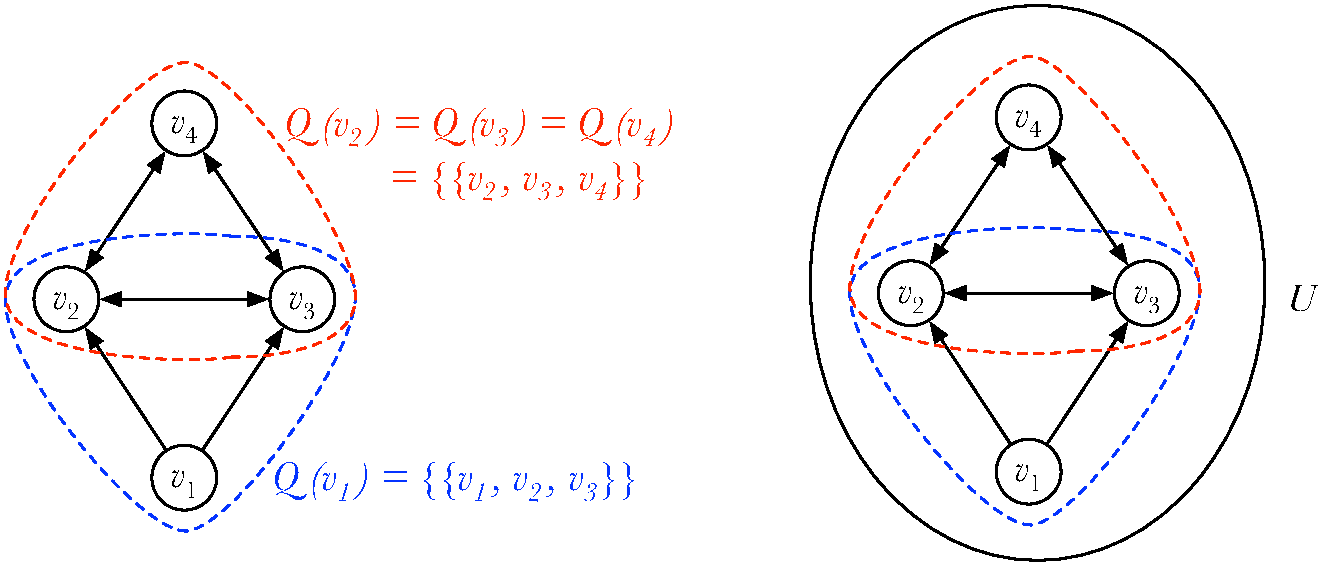
\includegraphics[width=15 cm]{Figures/example1}
\caption{\bf \small Example 1. L: a) The slices of this network. R: b) The smallest quorum involving $v_1$. (After \cite{Mazieres2016})}
\label{fig:example1}
\end{figure}

In traditional, non-federated Byzantine systems all nodes have the same slices. Therefore, non-federated systems do not distinguish between slices and quorums:
\begin{align}
\forall v_i, v_j \in V, \qquad Q(v_i) = Q(v_j). \qquad\qquad \text{[BAS]} 
\end{align}
In our case, instead, in general we have that
\begin{align}
\forall v_i, v_j \in V, \qquad Q(v_i) \ne Q(v_j). \qquad\qquad \text{[FBAS]} 
\end{align}
The important point made by Mazi\`eres is that whereas BAS is not scalable, as exemplified by the huge CPU overhead the Bitcoin consensus protocol requires, FBAS is scalable.

\begin{center}
\small
\frame{\colorbox{light-gray}{\makebox[16.5cm]{\parbox{16.5cm}{
%\vspace{.2cm}
\begin{quote}
\textbf{Example 2}
It is worth discussing a second example from Mazi\`eres, as shown in Figure \ref{fig:example2}. The figure shows three new notational concepts:
\vspace{.3cm}
\begin{packed_item1}
\item a reflexive dependence arrow can be drawn explicitly
\item sets of nodes can be grouped explicitly into separate sets or tiers, and
\item the dependence arrows can carry specific labels.
\end{packed_item1}
\end{quote}

\begin{quote}
For example, the label on the reflexive arrow on the top tier indicates that at least 3 nodes are needed for consensus. According to the definitions above for the arrow directions, the top tier does not depend on the tiers below, and it is precisely for this reason that it is the `top' tier. The label on the arrow between the middle and top tiers indicates that the slice of any one node from the middle tier is composed of itself plus any two of the tier above. The slice of either $v_9$ or $v_{10}$ is composed of itself plus any two nodes from the middle tier. Since each of these, in turn, depends on any two of the nodes of the top tier, neither such slice can be a quorum. A quorum involving either $v_9$ or $v_{10}$ will have at least 5 and at most 7 nodes. A quorum involving \emph{both} $v_9$ and $v_{10}$, on the other hand, will have at least 6 and at most all 10 nodes.
\end{quote}
\vspace{-.5cm}
\begin{figure}[H]
\centering
\captionsetup{width=11cm}
\frame{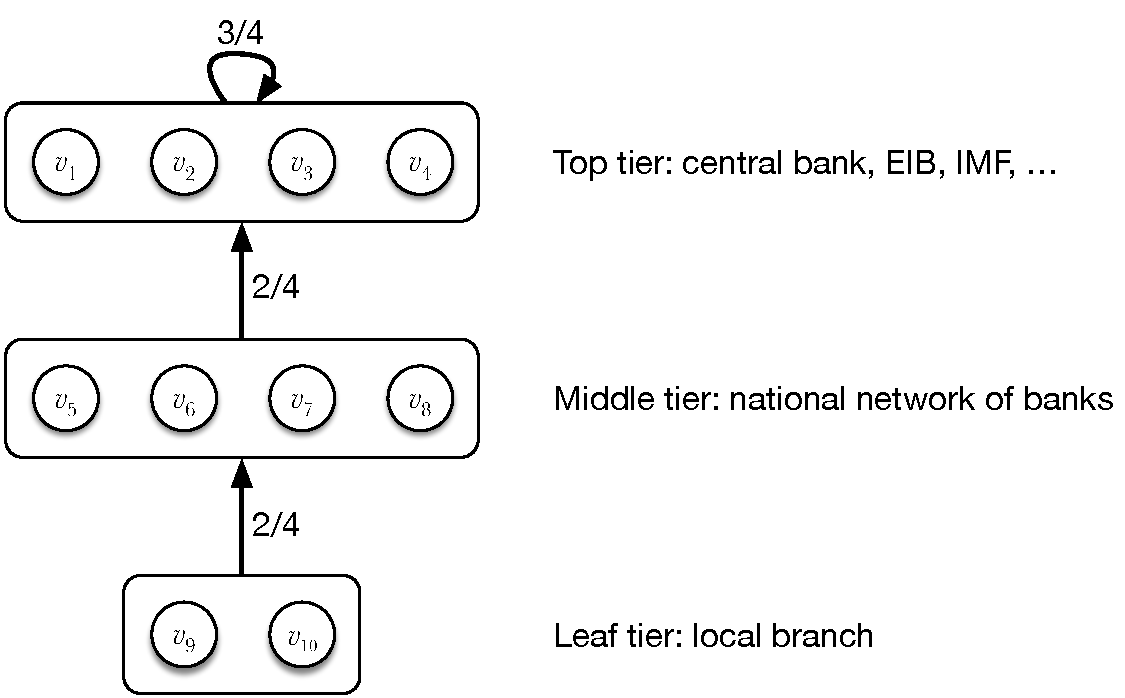
\includegraphics[width=11 cm]{Figures/example2}}
\caption{\bf \small Three-tier network (After \cite{Mazieres2016})}
\label{fig:example2}
\end{figure}

\begin{quote}
In Figure \ref{fig:example2} the top tier according to Mazi\`eres could be composed by a number of global financial institutions. The middle tier could be sets of banks operating at national level, with a single such set corresponding to a single country shown here. The bottom tier would be a single branch office, with the nodes inside representing individual customer accounts.
\end{quote}

\vspace{-.5cm}
\begin{figure}[H]
\centering
\captionsetup{width=15cm}
\frame{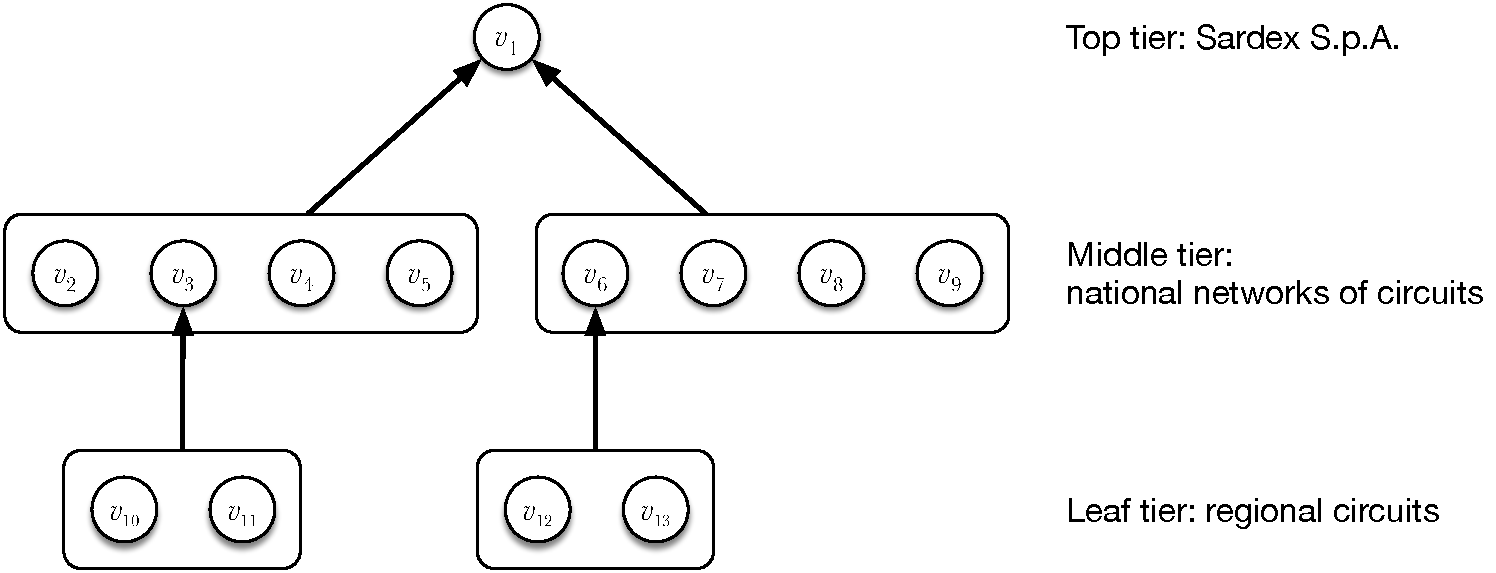
\includegraphics[width=15 cm]{Figures/example2_Sardex}}
\caption{\bf \small Possible mapping to INTERLACE circuit architecture. (After \cite{Mazieres2016})}
\label{fig:example2_Sardex}
\end{figure}
}}}}
\end{center}

\begin{center}
\small
\frame{\colorbox{light-gray}{\makebox[16.5cm]{\parbox{16.5cm}{
%\vspace{.2cm}

\begin{quote}
%\vspace{-.3cm}
In Figure \ref{fig:example2_Sardex}, on the other hand, the top tier would be only the single Sardex S.p.A.\ company. The middle tier could be composed by different national jurisdictions, each of which containing a set of circuits; the figure shows two such jurisdictions corresponding to two different countries. The bottom tier would then correspond to separate individual circuits, with the nodes corresponding to individual company accounts. There are no labels on the arrows because the dependence is to a specific node in every case, generating a centralized hierarchical network.
\end{quote}
\vspace{.2cm}
}}}}
\end{center}

Although the architecture of Figure \ref{fig:example2_Sardex} may correspond to an initial implementation of the INTERLACE platform, it does not make use of the distribution capability of the Stellar consensus protocol, so let's proceed with the development of the protocol to see what will become possible.

\subsection{Safety and Liveness}
Nodes can be either well-behaved or ill-behaved. A well-behaved node chooses sensible quorum slices and obeys the protocol, including responding (eventually) to all requests. Ill-behaved nodes suffer Byzantine failure, meaning that they behave arbitrarily due for example to a malicious modification of the software, or may have crashed. The goal of FBAS is to ensure that all well-behaved nodes externalize the same values in spite of such ill-behaved nodes.
\begin{quote}
\vspace{-0.6cm}
\small
\begin{defin}
Two nodes in a set $V$ are \emph{\textbf{divergent}} if they externalize different values to the same slot. A set $V$ of nodes in a FBAS is \emph{\textbf{safe}} if no two of its elements (nodes) externalize different values for the same slot.
\end{defin}
\begin{defin}
A node $v \in V$ is \emph{\textbf{blocked}} if it is in some dead-end state from which consensus is no longer possible. A node $v \in FBAS$ has \emph{\textbf{liveness}} if it can externalize new values without the participation of any failed or ill-behaved nodes.
\end{defin}
\begin{defin}
Nodes that enjoy both safety and liveness are called \emph{\textbf{correct}}. Nodes that are not correct have \emph{\textbf{failed}}.
\end{defin}
\end{quote}
Thus, nodes without liveness are blocked, whereas nodes without safety are divergent. Figure \ref{fig:correct} shows the set inclusion relationships between these different kinds of nodes in a set $V$. The reason a divergent or blocked node is shown under the well-behaved category even though it has failed is that, unlike ill-behaved nodes, it may have started as a correct node but may fail if its choice of slice causes it to wait indefinitely for messages from an ill-behaved node (this makes it {\bf blocked}) or, worse, if its state is maliciously modified by messages from an ill-behaved node (this makes it {\bf divergent}). Thus, the reason divergent nodes are a subset of the blocked nodes is that an attack that violates safety is strictly more powerful that one that violates only liveness.

\begin{figure}[h]
\centering
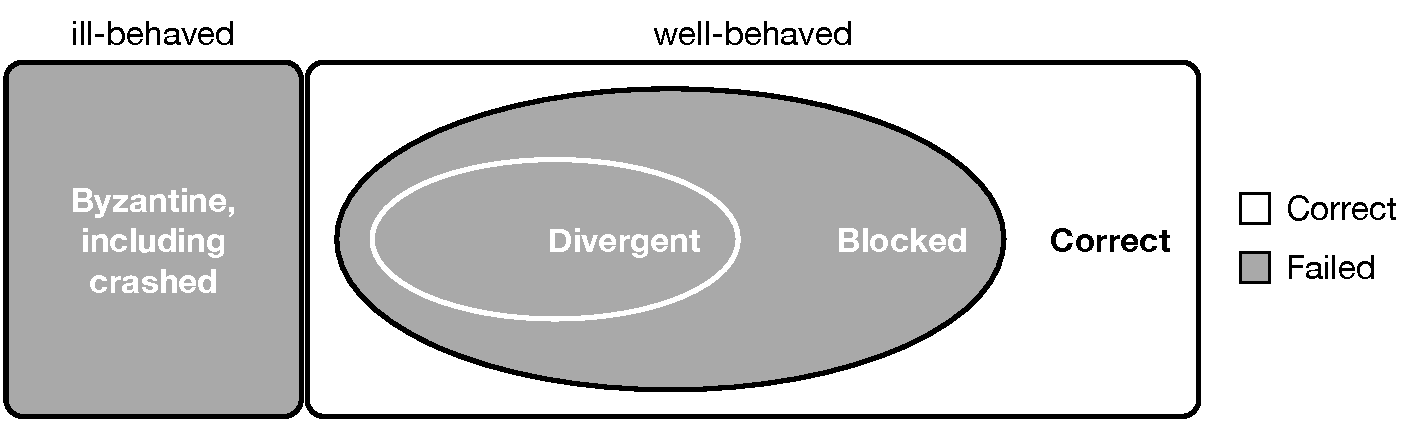
\includegraphics[width=14 cm]{Figures/correct}
\caption{\bf \small Set inclusion relationships between node categories. (After \cite{Mazieres2016})}
\label{fig:correct}
\end{figure}

Mazi\`eres explains that the above definition of liveness is weak because it only says that a node \emph{can} externalize, not that it \emph{will} or \emph{must}. As a consequence, there is a possibility for consensus to be forever delayed by, for example, preemptive reordering of the transactions. It is not clear whether this issue matters in the case of INTERLACE since we will not implement a completely decentralized system: some level of centralized control is likely to remain. Mazi\`eres in any case provides relevant references that can be consulted if this issue needs to be analysed in depth and resolved in some robust way.

\subsubsection{Optimal Resilience: Quorum Intersection and Dispensable Sets}
As is commonly assumed for asynchronous systems, messages between well-behaved nodes are eventually delivered, but can otherwise be delayed indefinitely or reordered arbitrarily. This section starts becoming more involved because it addresses the following non-trivial question: Given a specific $(V, Q)$ and a subset of $V$ that is ill-behaved, what are the best levels of safety and liveness that a FBAS can guarantee in an arbitrary network?
\begin{quote}
\vspace{-0.6cm}
\small
\begin{defin}
\label{QI}
A FBAS has \emph{\textbf{quorum intersection}} iff any two of its quorums share at least one node.\footnote{The term `iff' means `if and only if'. It implies that the causal dependence works in both directions, in contrast to merely `if' which works only in the reverse direction. In symbols, `A iff B' is written $A \Leftrightarrow B$, whereas `A if B' is written $B \Rightarrow A$ and is also read as `B implies A'.} In other words, $\forall U_i, U_j \in FBAS, U_i \cap U_j \ne 0$, where $i$ and $j$ range over the number of quorums for a given FBAS.
\end{defin}
\end{quote}

Therefore, when a FBAS has many quorums, quorum intersection (QI) fails when \textbf{\textit{any two}} do not intersect. We remind the reader that $Q(v_i)$ is just the set of slices of a given node $v_i$ and, depending on the slices of all the other nodes $v_j \in Q(v_i)$, may or may not be a quorum $U \subseteq V$. Thus, although in the simple examples that follow each $Q(v)$ is a quorum, this is by no means the case in general.

\begin{figure}[h]
\centering
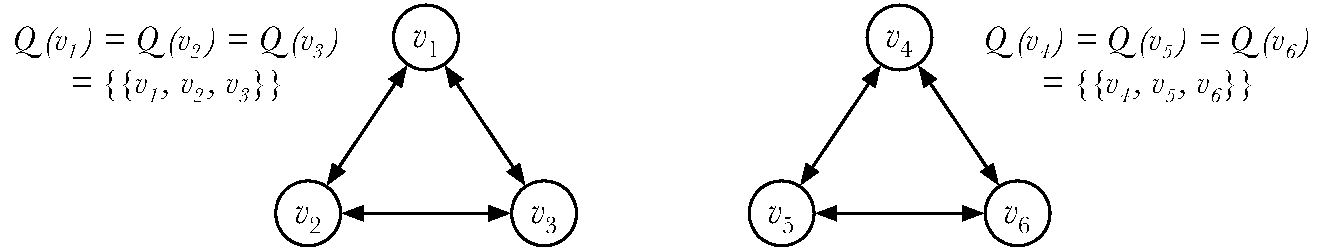
\includegraphics[width=15 cm]{Figures/QI1}
\caption{\bf \small A set of nodes without QI. (After \cite{Mazieres2016})}
\label{fig:QI1}
\end{figure}

Figure \ref{fig:QI1} shows a system of 6 nodes that lacks QI, since the function $Q$ allows two quorums on the set of 6 nodes that do not intersect. Mazi\`eres says that the two quorums can separately agree on contradictory statements. In other words, since $v_5$ cannot communicate with $v_1$, it could say something different from what $v_1$ is saying for a given slot. Mazi\`eres says that the whole set of all nodes $\{ v_1, \cdots, v_6 \}$ is \emph{also} a quorum, which in this case we can call $U$, and it intersects the other two. Is this true? If we look back at the definition of a quorum (Definition \ref{quorum}), we can verify that yes, it is correct because each node has a slice that is part of $U$. So this is an example of a system that has multiple quorums but two of them do not intersect and, therefore, the system does not have QI. We can believe that there is no certainty that $v_1$ can contradict or agree with $v_5$ even though they both belong to $U$.

\begin{figure}[h]
\centering
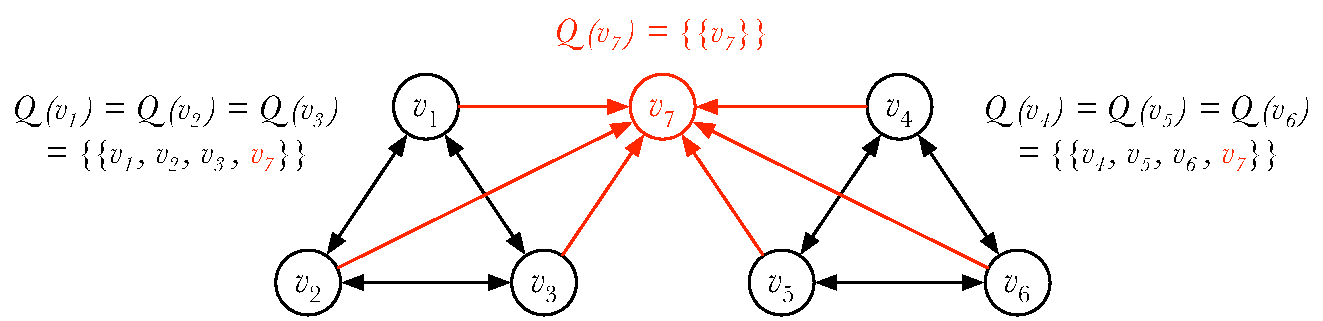
\includegraphics[width=15 cm]{Figures/QI2}
\caption{\bf \small A set of nodes with QI. (After \cite{Mazieres2016})}
\label{fig:QI2}
\end{figure}

Safety cannot be guaranteed because such a system can operate like two separate FBAS systems that do not communicate. However, safety may not be possible even in a system with QI, like the one shown in Figure \ref{fig:QI2}, if the intersecting node is ill-behaved. If $v_7$ makes inconsistent statements to the left and right quorums they are as good as disconnected. Therefore, safety can be guaranteed only if the well-behaved nodes have QI; or, put otherwise, a FBAS $(V, Q)$ can survive Byzantine failure by a set $B \subseteq V$ iff $(V, Q)$ has QI after deleting the nodes in $B$ from $V$ and from all slices in $Q$. 

More formally,
\begin{quote}
\vspace{-0.6cm}
\small
\begin{defin}
\label{delete}
If $(V, Q)$ is a FBAS and $B \subseteq V$ is a set of nodes, then to \emph{\textbf{delete}} $B$ from $(V, Q)$, written $(V, Q)^B$, means to compute the modified $(V \setminus B, Q^B)$, where
\begin{align}
Q^B(v) = \{ q \setminus B\ |\ q \in Q(v) \},		\qquad \forall v \in V \setminus B.
\end{align}
\end{defin}
\end{quote}
It is the responsibility of each node $v$ to ensure that $Q(v)$ does not violate QI. From Mazi\`eress paper it is not clear {\bf how}, however. Be that as it may, assume that Figure \ref{fig:QI2} evolved from the 3-node FBAS $\{ v_1, v_2, v_3 \}$ to a system that includes also $\{ v_4, v_5, v_6 \}$. Assume now that $\{ v_4, v_5, v_6 \}$ are malicious such that they choose slices that do not satisfy QI. But $Q(v)$ is meaningless for a malicious node. That's why the necessary condition for safety, QI after deleting ill-behaved nodes, is unaffected by the slices of ill-behaved nodes. The system $(V, Q)^{ \{ v_4, v_5, v_6 \} }$ restores QI for $\{ v_1, v_2, v_3 \}$. Note that we have not yet said how such deletion takes place. For now we just say that the protocol must guarantee safety for $\{ v_1, v_2, v_3 \}$ without these nodes having to know that $\{ v_4, v_5, v_6 \}$ are malicious.

Turning now to dispensable sets or DSets, the safety and liveness of the nodes outside a DSet can  be guaranteed regardless of the behaviour of the nodes inside the DSet.
\begin{quote}
\vspace{-0.6cm}
\small
\begin{defin}
\label{dset}
Let $(V, Q)$ be a FBAS and $B \subseteq V$ be a set of nodes. We say that $B$ is a dispensable set or a \emph{\textbf{DSet}} iff:
\begin{packed_item1}
\item $(V, Q)^B$ has QI \qquad\qquad\qquad\qquad\ (Intersection)
\item $V \setminus B$ is a quorum OR $B = V$ \qquad (Availability)
\end{packed_item1}
\end{defin}
\end{quote}
As explained by Mazi\`eres, availability protects against nodes in $B$ not replying to requests or impeding other nodes' progress. QI protects against nodes in $B$ making contradictory assertions that enable other nodes to externalize inconsistent values for the same slot. These two threats depend on slice size in opposite ways: greater slices increase the chance for QI, but also the chance that they will contain failed nodes, impacting availability. Smaller slices decrease the chance of failed nodes, but also the likelihood of having QI.

The smallest DSet containing all ill-behaved nodes may contain also well-behaved nodes, if they depend on the ill-behaved ones. For example, in Figure \ref{fig:example2} if $v_5$ and $v_6$ are ill-behaved the smallest DSet would need to include also $v_9$ and $v_{10}$ since the lowest tier depends on any 2 of the nodes in the middle tier, and so it may depend on the two that are ill-behaved.
\begin{quote}
\vspace{-0.6cm}
\small
\begin{defin}
\label{intact}
A node $v \in FBAS$ is \emph{\textbf{intact}} iff $\exists\  DSet\  B$ containing all ill-behaved nodes and such that $v \notin B$.
\end{defin}
\begin{defin}
\label{befouled}
A node $v \in FBAS$ is \emph{\textbf{befouled}} iff it is not intact.
\end{defin}
\begin{theorem}
\label{theorem1}
Let $U$ be a quorum in FBAS $(V, Q)$. Let $B \subseteq V$, so that $B$ is not necessarily a slice of $U$. And let $U' = U \setminus B$. If $U' \neq \emptyset$, then $U'$ is a quorum in $(V, Q)^B$.
\end{theorem}
\begin{proof}
First, as shown in Figure \ref{fig:theorem1}A, since $U$ is a quorum, every $v \in U$ has a slice $q \in Q(v)$ such that $q \in U$:
\begin{align}
\exists q \in Q(v) | q\in U, \qquad \forall v \in U.
\end{align}
Second, as shown in Figure \ref{fig:theorem1}B, since $U' \subseteq U$, every $v \in U'$ has $q \in Q(v)$ such that $q \setminus B \subseteq U'$:
\begin{align}
\exists q \in Q^B(v) | q \in U', \qquad \forall v \in U'.
\end{align}
Therefore, $U'$ is a quorum in $(V, Q)^B$.
\end{proof}
\end{quote}

\begin{figure}[H]
\centering
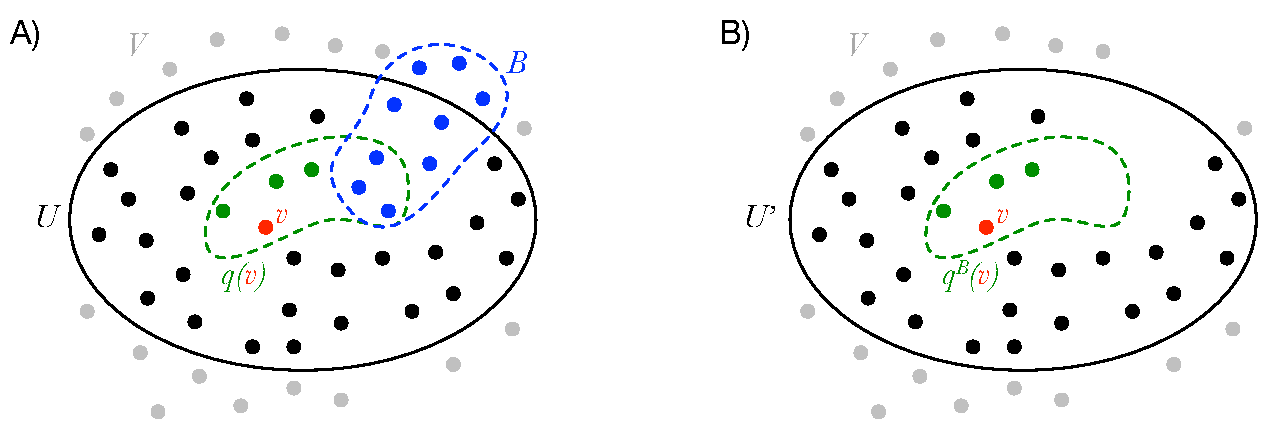
\includegraphics[width=15 cm]{Figures/theorem1}
\caption{\bf \small A) Quorum $U \subseteq V$ with set $B \subseteq V$. B) $U' = U \setminus B$ and $q^B(v) = q(v) \setminus B$.}
\label{fig:theorem1}
\end{figure}

The next theorem is far from obvious.
\begin{quote}
%\vspace{-0.6cm}
\small
\begin{theorem}
%\vspace{-0.4cm}
\label{theorem2}
If $B_1$ and $B_2$ are DSets in a PBAS $(V, Q)$ that has QI, then $B = B_1 \cap B_2$ is a DSet too.
\end{theorem}

\begin{figure}[h]
\centering
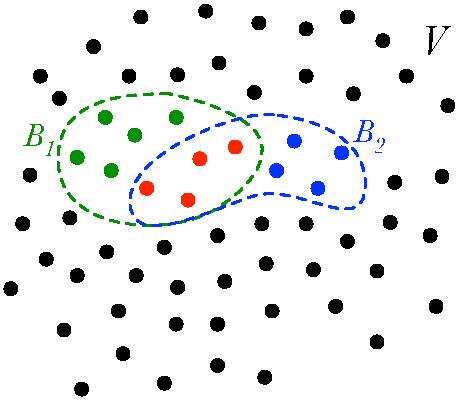
\includegraphics[width=5 cm]{Figures/Thm2_V}
\caption{\bf \small Visualization of a set of nodes $V$ with two\\ DSets $B_1$ and $B_2$ and their intersection in red}
\label{fig:Thm2_V}
\vspace{-0.5cm}
\end{figure}

\begin{proof}
Let $U_1 = V \setminus B_1$ and $U_2 = V \setminus B_2$ be two subsets of $V$ defined by taking away the two DSets in turn, as shown in Figure \ref{fig:Thm2_U1_U2}. Note that by Definition \ref{dset} both subsets have QI. By the same definition, both subsets are also quorums.

\begin{figure}[h]
\centering
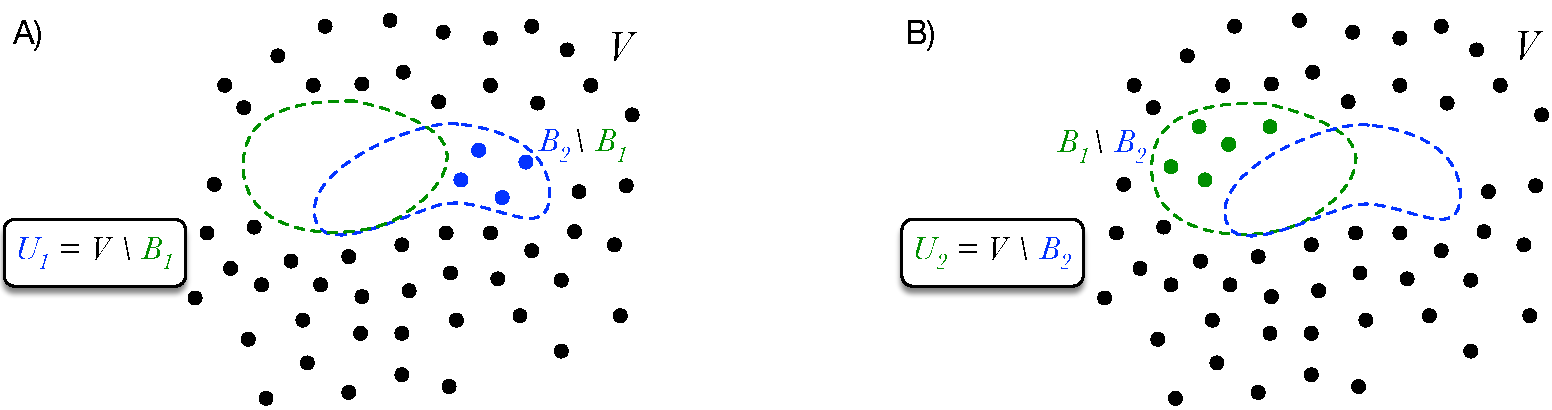
\includegraphics[width=16 cm]{Figures/Thm2_U1_U2}
\caption{\bf \small The two subsets $U_1$ and $U_2$}
\label{fig:Thm2_U1_U2}
\vspace{-0.4cm}
\end{figure}

\begin{case}
If $U_1 = \emptyset$, then $B_1 = V$ and $B = V \cap B_2 = B_2$, which is a DSet.
%\vspace{-0.4cm}
\end{case}
\begin{case}
Similarly, if $U_2 = \emptyset$, then $B_2 = V$ and $B = B_1 \cap V = B_1$, which is a DSet.
%\vspace{-0.4cm}
\end{case}
\begin{case}
If we are not at these two extremes, as just stated above by quorum availability $U_1$ and $U_2$ are both quorums in $(V, Q)$. Also, the quorum definition \ref{quorum} implies that $U_1 \cup U_2$ (which also equals $V \setminus B$) is also a quorum (see Figure \ref{fig:Thm2_U1_U_U2}A). Therefore, $V \setminus B$ is a quorum. Therefore, $B_1 \cap B_2$ satisfies availability in $V$ despite $B$. This proves the {\bf availability} condition of a DSet, i.e.\ availability despite $B$. Proving {\bf QI} despite $B$ requires quite a bit more work.

\begin{figure}[h]
\centering
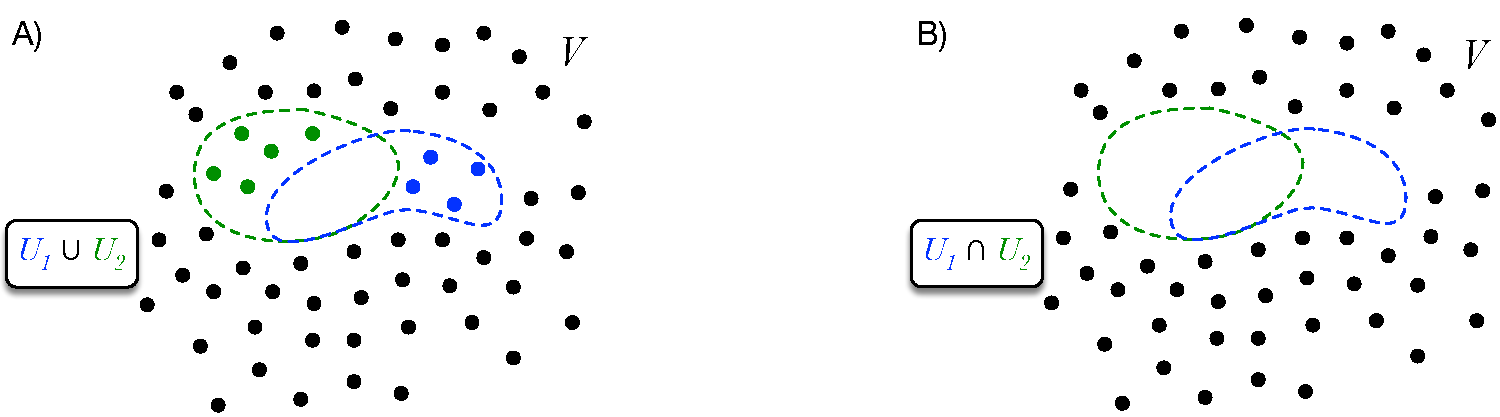
\includegraphics[width=16 cm]{Figures/Thm2_U1_U_U2}
\caption{\bf \small Union and intersection of the two subsets $U_1$ and $U_2$}
\label{fig:Thm2_U1_U_U2}
\end{figure}

Let $U = U_1 \cap U_2$ (see Figure \ref{fig:Thm2_U1_U_U2}B). Note that $U$ also equals $U_2 \setminus B_1$  and $U_1 \setminus B_2$. By the definition of QI (Definition \ref{QI}), $U_1 \cap U_2 \ne \emptyset$. Then by Theorem \ref{theorem1} $U_1 \cap U_2 = U_2 \setminus B_1$ is a quorum in $(V, Q)^{B_1}$. In other words, Figure \ref{fig:Thm2_U1_U_U2}B is a quorum in Figure \ref{fig:Thm2_U1_U2}A.

\vspace{0.3cm}
$*$Let $U_a$ and $U_b$ be two quorums in $(V, Q)^B = U_1 \cup U_2$. We begin the analysis by working with $U_a$, and repeat the argument later for $U_b$.
\vspace{0.3cm}
\begin{packed_item1}
\item If $U_a \setminus B_1 = \emptyset$, $U_a$ must be at most $\subseteq B_1$ (but not include $B$, by construction)
\item Similarly, If $U_a \setminus B_2 = \emptyset$, $U_a$ must be at most $\subseteq B_2$ (but not include $B$, by construction)
\item If $U_a \setminus B_1 = \emptyset$ {\bf AND} $U_a \setminus B_2 = \emptyset$, then $U_a = \emptyset$.
\end{packed_item1}
\vspace{0.3cm}

Now whether or not $B_1$ and $B_2$ are quorums is not relevant to the argument since they are DSets by assumption. They are sets we wish to ignore. Therefore, the cases above are not of interest and are irrelevant. Therefore, we are only interested in the two cases
\begin{align}
U_a \setminus B_1 \ne \emptyset \qquad \text{\bf OR} \qquad U_a \setminus B_2 \ne \emptyset.
\end{align}

This implies that there are now three possibilities for $U_a$:
\vspace{0.3cm}
\begin{packed_enumerate}
\item $U_a \setminus B_1$ is a quorum in $\big( (V, Q)^B \big)^{B_1} = (V, Q)^{B_1}$
\item $U_a \setminus B_2$ is a quorum in $\big( (V, Q)^B \big)^{B_2} = (V, Q)^{B_2}$
\item Both, i.e.\ the quorum is outside of both $B_1$ and $B_2$.
\end{packed_enumerate}
\vspace{0.3cm}
What we show next is that if 1) is true, then 2) is true too, and vice versa. Therefore, since we have ruled out all other possibilities, the next few lines will show that the \emph{only} possibility left is 3).

\vspace{0.3cm}
If 1) is true, then $(U_a \setminus B_1) \cap U \ne \emptyset$, by QI of $(V, Q)^{B_1}$.
In fact, since $B_1$ is a DSet by construction, $(V, Q)^{B_1}$ has QI. And since $(U_a \setminus B_1)$ and $U$ are both quorums, by definition of QI their intersection is not empty.
%%% The following is NOT the reason why $(V, Q)^{B_1}$ has QI. It is merely consistent with the fact that it does. In other words, it is necessary but not sufficient. Therefore, I am commenting this out:
%\vspace{0.3cm}
%\makebox[\textwidth][c]{
%\begin{minipage}{.5\textwidth}
%Let us revisit why:\\
%-- $U = U_1 \cap U_2 = (V \setminus B_1) \cap (V \setminus B_2) = V \setminus (B_1 \cup B_2)$.\\
%-- Therefore, $U \subseteq V \setminus B_1$\\
%-- We have already seen that $U$ is a quorum in $(V, Q)^{B_1}$\\
%-- $U_a \setminus B_1$ is a quorum by Theorem \ref{theorem1}\\
%-- Therefore, $(V, Q)^{B_1}$ has QI.
%\end{minipage}
%}
Now, $(U_a \setminus B_1) \cap U$ happens to equal $(U_a \setminus B_1) \setminus B_2$. Therefore, $(U_a \setminus B_1) \setminus B_2 \ne \emptyset$. If that is the case, then even more
$U_a \setminus B_2 \ne \emptyset$. Therefore, by Theorem \ref{theorem1} $U_a \setminus B_2$ is a quorum in $(V, Q)^{B_2}$.

\vspace{0.3cm}
Similarly, if 2) is true, then $(U_a \setminus B_2) \cap U \ne \emptyset$, by QI of $(V, Q)^{B_2}$, since $B_2$ is also a DSet. Since $(U_a \setminus B_2) \cap U = (U_a \setminus B_2) \setminus B_1$, $(U_a \setminus B_2) \setminus B_1 \ne \emptyset$, and $U_a \setminus B_1 \ne \emptyset$ either. Therefore, by Theorem \ref{theorem1} $U_a \setminus B_1$ is a quorum in $(V, Q)^{B_1}$.

\vspace{0.3cm}
Therefore, 3) is the only possibility left. Knowing this helps a global understanding of all the possibilities, but we have actually done more work than was strictly necessary to prove the theorem. All we need to focus on is 1): $U_a \setminus B_2$ is a quorum in $(V, Q)^{B_2}$.

\vspace{0.3cm}
Now go back to $*$ and follow the same argument for $U_b$. Look at the possibility 1) that
$U_b \setminus B_1$ is a quorum. Following the same argument we can show that this implies that $U_b \setminus B_2$ is a quorum in $(V, Q)^{B_2}$. But then, by QI despite $B_2$, we necessarily have that
\begin{align}
(U_a \setminus B_2) \cap (U_b \setminus B_2) \ne \emptyset.
\end{align}
If that's true, $U_a \cap U_b \ne \emptyset$ is even more so. Since $U_a$ and $U_b$ are any two quorums in $(V, Q)^B$, we have proven QI despite $B$. Hence $B$ is a DSET.
\end{case}
\vspace{-0.5cm}
\end{proof}
\end{quote}

The above theorem may seem ``much ado about nothing'', but in fact it has shown a rather important general fact, namely that DSets are closed under intersection. We use this fact immediately, in the next theorem.



\begin{quote}
\small
\begin{theorem}
\label{theorem3}
In a FBAS with QI, the set of befouled nodes is a DSet.
\end{theorem}
\begin{proof}
In the definition of DSet we did not specify whether the nodes contained in a DSet were ill-behaved, blocked, divergent, or correct. We only said that what's left after we take a DSet is a quorum and, in addition, it has QI (if it happens to contain other quorums).

\vspace{0.3cm}
Now let a FBAS contain an arbitrary number of DSets, such that each DSet may contain a number of ill-behaved nodes. Let $B_{min}$ be the specific intersection of these DSets that contains all the ill-behaved nodes. According to Definition \ref{intact}, a node $v$ is intact iff $v \notin B_{min}$. Therefore, $B_{min}$ is the set of befouled nodes. By Theorem \ref{theorem2}, $B_{min}$ is a DSet.
\end{proof}
\end{quote}











\end{document}